%\documentclass[12pt]{article}

\questionheader{ex:s2.9}


%%%%%%%%%%%%%%%%%%
\subsection*{\Conceptual}
%%%%%%%%%%%%%%%%%%

%%%%%%%%%%%%%%%%%%%%%%%%%%%%%%%%
\begin{question}[M200 2016D] %2
\begin{enumerate}[(a)]
\item
Some level curves of a function $f(x,y)$ are plotted in the $xy$--plane 
below. 

\begin{center}
     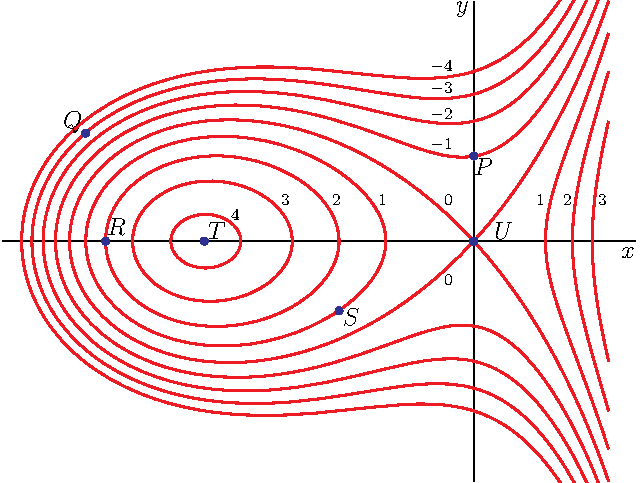
\includegraphics[scale=1.4]{OE16D_2a.pdf}
\end{center}

For each of the four statmements below, circle the letters of
\textbf{all} points in the diagram where the situation applies.
For example, if the statement were ``These points are on the $y$--axis'', you would circle both $P$ and $U$, but none of the other letters.
You may assume that a local maximum occurs at point $T$. 
\begin{align*}
\text{(i) }& \vnabla f\text{ is zero} & &\text{P R S T U} \\
\text{(ii) }& \text{ $f$ has a saddle point} & &\text{P R S T U} \\
\text{(iii) }& \text{ the partial derivative $f_y$ is positive} & &\text{P R S T U} \\
\text{(iv) }& \text{ the directional derivative of $f$ in the 
                 direction $\llt 0,-1\rgt$ is} & &\text{P R S T U} \\[-0.07in]
          & \text{ negative} & & 
\end{align*}


\item
The diagram below shows three ``$y$ traces'' of a graph $z=F(x,y)$ plotted
on $xz$--axes. (Namely the intersections of the surface  $z=F(x,y)$ with the 
three planes ($y=1.9$, $y=2$, $y=2.1$). For each statement below, circle the
correct word.
\begin{align*}
\text{(i) }& \text{ the first order partial derivative $F_x(1,2)$ is} & &\text{positive/negative/zero (circle one)} \\
\text{(ii) }& \text{ $F$ has a critical point at $(2,2)$ } & 
         &\text{true/false (circle one)} \\
\text{(iii) }& \text{ the second order partial derivative $F_{xy}(1,2)$ is} & &\text{positive/negative/zero (circle one)} 
\end{align*}

\begin{center}
     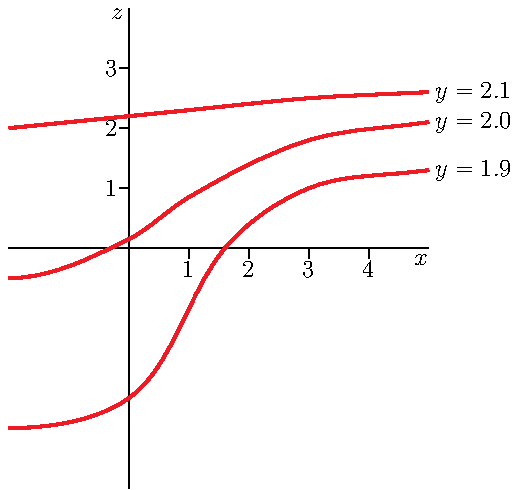
\includegraphics{OE16D_2b.pdf}
\end{center}
\end{enumerate}
\end{question}

%\begin{hint}
%
%\end{hint}

\begin{answer}
(a) (i) $T$, $U$

(a) (ii) $U$

(a) (iii) $S$

(a) (iv) $S$

(b) (i) $F_x(1,2)>0$

(b) (ii) $F$ does \emph{not} have a critical point at $(2,2)$.

(b) (iii) $F_{xy}(1,2)<0$
\end{answer}

\begin{solution}
a) (i) $\vnabla f$ is zero at critical points. 
        The point $T$ is a local maximum and the point $U$ is
        a saddle point. The remaining points $P$, $R$, $S$, are not
        critical points.

(a) (ii) Only $U$ is a saddle point. 

(a) (iii) We have $f_y(x,y)>0$ if $f$ increases as you move vertically upward
          through $(x,y)$. Looking at the diagram, we see
\begin{align*}
f_y(P) <0\qquad
f_y(Q) <0\qquad
f_y(R) =0\qquad
f_y(S) >0\qquad
f_y(T) =0\qquad
f_y(U) =0
\end{align*}
So only $S$ works.

(a) (iv) The directional derivative of $f$ in the direction $\llt 0,-1\rgt$
           is $\vnabla f\cdot \llt 0,-1\rgt =-f_y$. It is negative if and
           only if $f_y>0$. So, again, only $S$ works.

(b) (i) The function $z=F(x,2)$ is increasing at $x=1$,
     because the $y=2.0$ graph in the diagram has positive slope at $x=1$.
     So $F_x(1,2)>0$.

(b) (ii) The function $z=F(x,2)$ is also increasing (though slowly) at $x=2$,
     because the $y=2.0$ graph in the diagram has positive slope at $x=2$.
     So $F_x(2,2)>0$. So $F$ does \emph{not} have a critical point
     at $(2,2)$.


(b) (iii) From the diagram the looks like 
                $F_x(1,1.9) > F_x(1,2.0) > F_x(1,2.1)$.
      That is, it looks like the slope of the $y=1.9$ graph at $x=1$
             is larger than the slope of the $y=2.0$ graph at $x=1$,
             which in turn 
             is larger than the slope of the $y=2.1$ graph at $x=1$.
     So it looks like $F_x(1,y)$ decreases as $y$ increases through $y=2$,
     and consequently $F_{xy}(1,2)<0$.
\end{solution}


%%%%%%%%%%%%%%%%%%%%%%%%%%%%%%%%
\begin{question}
Find the high and low points of the surface $\ z=\sqrt{x^2+y^2}\ $ with $(x,y)$ 
varying over the square $\ |x|\le 1$, $|y|\le 1\ $. Discuss the values of 
$\ z_x,\ z_y\ $ there. Do not evaluate any derivatives in answering this 
question.
\end{question}

\begin{hint}
Interpret the height $\sqrt{x^2+y^2}$ geometrically.
\end{hint}

\begin{answer}
The minimum height is zero at $(0,0,0)$. The derivatives 
$z_x$ and $z_y$ do not exist there. 
The maximum height is $\sqrt{2}$ at $(\pm 1,\pm 1,\sqrt{2})$. 
There $z_x$ and $z_y$ exist but are not zero --- those points would 
not be the highest points if it were not for the restriction 
$|x|,|y|\le 1$.
\end{answer}

\begin{solution}
The height $\sqrt{x^2+y^2}$ at $(x,y)$ is the distance from $(x,y)$
to $(0,0)$. So the minimum height is zero at $(0,0,0)$. The surface is a 
cone. The cone has a point at $(0,0,0)$ and the derivatives 
$z_x$ and $z_y$ do not exist there. 
The maximum height is achieved when $(x,y)$ is as far as possible from
$(0,0)$. The highest points are at $(\pm 1,\pm 1,\sqrt{2})$. There 
$z_x$ and $z_y$ exist but are not zero. These points would not 
be the highest points if it were not for the restriction $|x|,|y|\le 1$.
\end{solution}

%%%%%%%%%%%%%%%%%%%%%%%%%%%%%%%%
\begin{question}
If $t_0$ is a local minimum or maximum of the smooth function $\ f(t)\ $
of one variable ($t$ runs over all real numbers) then $\ f'(t_0)=0.$
Derive an analogous necessary condition for $\vx_0$ to be a local minimum
or maximium of the smooth function $\ g(\vx)\ $ \textbf{restricted} to points on
the line $\ \vx=\va+t\vd\ .$ The test should involve the gradient 
of $g(\vx)$. 

\end{question}

\begin{hint}
Define $f(t)=g(\va+t\vd)$.
\end{hint}

\begin{answer}
$\vnabla g(\vx_0)\cdot\vd=0$, i.e. $\vnabla g(\vx_0)\perp\vd$, and $\vx_0=\va+t_0\vd$ for some $t_0$. 
The second condition is to ensure that $x_0$ lies on the line.
\end{answer}

\begin{solution}
 Define $f(t)=g(\va+t\vd)$ and determine $t_0$ by 
$\vx_0=\va+t_0\vd$. Then $f'(t)=\vnabla g(\va+t\vd)\cdot\vd$. 
To see this, write $\va=\llt a_1,a_2,a_3\rgt$ and $\vd=\llt d_1,d_2,d_3\rgt$.
Then 
\begin{equation*}
f(t)=g(a_1+td_1,a_2+td_2,a_3+td_3)
\end{equation*} 
So, by the chain rule,
\begin{align*}
f'(t) &= \pdiff{g}{x}(a_1+td_1,a_2+td_2,a_3+td_3)\,d_1
       +\pdiff{g}{y}(a_1+td_1,a_2+td_2,a_3+td_3)\,d_2 \\&\hskip2in
       +\pdiff{g}{z}(a_1+td_1,a_2+td_2,a_3+td_3)\,d_3 \\
     &=\vnabla g(\va+t\vd)\cdot\vd
\end{align*}
Then $\vx_0$ is a local
max or min of the restriction of $g$  to the specified line if and only
if $t_0$ is a local max or min of $f(t)$. If so, $f'(t_0)$  necessarily
vanishes. So if $\vx_0$ is a local
max or min of the restriction of $g$  to the specified line,
then $\vnabla g(\vx_0)\cdot\vd=0$, i.e. $\vnabla g(\vx_0)\perp\vd$, and $\vx_0=\va+t_0\vd$ for some $t_0$. 
The second condition is to ensure that $x_0$ lies on the line.
\end{solution}



%%%%%%%%%%%%%%%%%%%%%%%%%%%%
%\Instructions{Questions~\ref{prob_s1.0first} through \ref{prob_s1.0last} provide practice with.}
%%%%%%%%%%%%%%%%%%%%

%%%%%%%%%%%%%%%%%%
\subsection*{\Procedural}
%%%%%%%%%%%%%%%%%%

%%%%%%%%%%%%%%%%%%%%%%%%%%%%%%%%
\begin{question}[M200 2005D] %5
Let $z = f(x,y) = {(y^2 - x^2)}^2$.
\begin{enumerate}[(a)]
\item
Make a reasonably accurate sketch of the level curves in the $xy$--plane 
of $z = f(x,y)$ for $z = 0$, $1$ and $16$. Be sure to show the units 
on the coordinate axes.
\item
Verify that $(0,0)$ is a critical point for $z = f(x,y)$, and 
determine from part (a) or directly from the formula for $f(x,y)$ 
whether $(0, 0)$ is a local minimum, a local maximum or a saddle point.
\item
Can you use the Second Derivative Test to determine whether the 
critical point $(0, 0)$ is a local minimum, a local maximum or 
a saddle point? Give reasons for your answer.
\end{enumerate}

\end{question}

\begin{hint}
Write down the equations of specified level curves.
\end{hint}

\begin{answer}
(a)
\begin{center}
     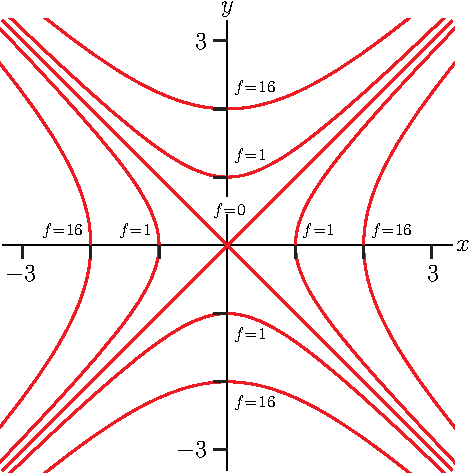
\includegraphics[scale=0.8]{OE05D_5.pdf}
\end{center}

(b) $(0,0)$ is a local (and also absolute) minimum.

(c) No. See the solutions.
\end{answer}

\begin{solution}
(a) 
\begin{itemize}
\item 
The level curve $z=0$ is $y^2-x^2=0$, which is the pair
of $45^\circ$ lines $y=\pm x$. 
\item
When $C>0$, the level curve  
$z=C^4$ is ${(y^2-x^2)}^2=C^4$, which is the pair of hyperbolae 
$y^2-x^2=C^2$, $y^2-x^2=-C^2$ or 
\begin{equation*}
y=\pm\sqrt{x^2+C^2}\qquad x=\pm\sqrt{y^2+C^2}
\end{equation*}
The hyperbola  $y^2-x^2=C^2$ crosses the $y$--axis (i.e. the line $x=0$) 
at $(0,\pm C)$.
The hyperbola  $y^2-x^2=-C^2$ crosses the $x$--axis (i.e. the line $y=0$) 
at $(\pm C,0)$.
\end{itemize}
Here is a sketch showing the level curves $z=0$, $z=1$ (i.e. $C=1$),
and $z=16$ (i.e. $C=2$).

\begin{center}
     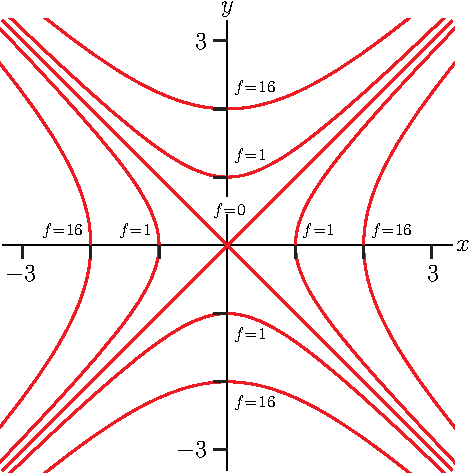
\includegraphics{OE05D_5.pdf}
\end{center}

(b)
As $f_x(x,y)=-4x(y^2-x^2)$ and $f_y(x,y)=4y(y^2-x^2)$, we have 
$f_x(0,0) = f_y(0,0) = 0$ so that $(0,0)$ is a critical point. Note that 
\begin{itemize}
\item
$f(0,0)=0$, 
\item
$f(x,y)\ge 0$ for all $x$ and $y$.
\end{itemize}
So $(0,0)$ is a local (and also absolute) minimum.

(c) 
Note that
\begin{alignat*}{3}
f_{xx}(x,y) &=-4y^2+12x^2\qquad&
         f_{xx}(x,y)&=0 \\
f_{yy}(x,y) &= 12y^2-4x^2\qquad&
         f_{yy}(x,y)&=0 \\
f_{xy}(x,y) &=-8xy\qquad&
         f_{xx}(x,y)&=0 \\
\end{alignat*}
As 
$
f_{xx}(0,0)f_{yy}(0,0)-f_{xy}(0,0)^2=0
$,
the Second Derivative Test (Theorem \eref{CLP200}{thm second deriv test} 
in the CLP-3 text) tells us absolutely nothing.
\end{solution}

%%%%%%%%%%%%%%%%%%%%%%%%%%%%%%%%
\begin{question}[M200 2006A] %3
Use the Second Derivative Test to find all values of the constant $c$ 
for which the function $z = x^2 + cxy + y^2$ has a saddle point at $(0,0)$.
\end{question}

%\begin{hint}
%
%\end{hint}

\begin{answer}
$|c|>2$
\end{answer}

\begin{solution}
Write $f(x,y) = x^2 +cxy +y^2$. Then
\begin{align*}
f_x(x,y)&= 2x+cy & f_x(0,0) = 0 \\
f_y(x,y)&= cx+2y & f_y(0,0) = 0 \\
f_{xx}(x,y) &= 2 \\
f_{xy}(x,y) &= c \\
f_{yy}(x,y) &= 2
\end{align*}
As $f_x(0,0)=f_y(0,0)=0$, we have that $(0,0)$ is always a critical point
for $f$. According to the Second Derivative Test, $(0,0)$ is also a saddle point
for $f$ if
\begin{align*}
f_{xx}(0,0) f_{yy}(0,0) - f_{xy}(0,0)^2 <0
\iff 4-c^2 <0
\iff |c|>2
\end{align*}

As a remark, the Second Derivative Test provides no information 
when the expression
$f_{xx}(0,0) f_{yy}(0,0) - f_{xy}(0,0)^2 =0$, i.e. when $c=\pm 2$.
But when $c=\pm 2$,
\begin{equation*}
f(x,y) =  x^2 \pm 2xy + y^2 =(x\pm y)^2
\end{equation*}
and $f$ has a local minimum, not a saddle point, at $(0,0)$.
\end{solution}


%%%%%%%%%%%%%%%%%%%%%%%%%%%%%%%%
\begin{question}[M200 2006D] %3a

\end{question}
Find and classify all critical points of the function
\begin{equation*}
f(x, y) = x^3 - y^3 - 2xy + 6.
\end{equation*}
%\begin{hint}
%
%\end{hint}

\begin{answer}
\renewcommand{\arraystretch}{1.3}
     \begin{tabular}{|c|c|c|c|}
     \hline
    $\Atop{\text{critical}}{\text{point}}$ & type \\    
    \hline
     $(0,0)$ & saddle point  \\ \hline
     $\left(-\frac{2}{3},\frac{2}{3}\right)$ & local max \\  \hline
     \end{tabular}
\renewcommand{\arraystretch}{1.0}
\end{answer}

\begin{solution}
To find the critical points we will need the gradient of $f$, and to 
apply the second derivative test of 
Theorem \eref{CLP200}{thm second deriv test} in the CLP-3 text 
we will need all second order partial derivatives. So we need all 
partial derivatives of $f$ up to order two.
Here they are.
\begin{alignat*}{3}
f&=x^3 - y^3 - 2xy + 6 \hidewidth\\
f_x&=3x^2-2y   & f_{xx}&=6x \qquad & f_{xy}&= -2\\
f_y&=-3y^2-2x \qquad & f_{yy}&=-6y\qquad & f_{yx}&= -2
\end{alignat*}
The critical points are the solutions of
\begin{equation*}
f_x=3x^2-2y=0   \qquad
f_y=-3y^2-2x = 0
\end{equation*}
Substituting $y=\frac{3}{2}x^2$, from the first equation, into the
second equation gives
\begin{align*}
-3\left(\frac{3}{2}x^2\right)^2-2x =0
&\iff -2x\left(\frac{3^3}{2^3}x^3+1\right)=0 \\
&\iff x=0,\ -\frac{2}{3}
\end{align*}
So there are two critical points: $(0,0)$, 
        $\left(-\frac{2}{3},\frac{2}{3}\right)$.


The classification is
\begin{center}
\renewcommand{\arraystretch}{1.3}
     \begin{tabular}{|c|c|c|c|}
     \hline
    $\Atop{\text{critical}}{\text{point}}$  & $f_{xx}f_{yy}-f_{xy}^2$ & 
                                                          $f_{xx}$ & type \\    
    \hline
     $(0,0)$  & $0\times 0 -(-2)^2 < 0$ &   & saddle point  \\ \hline
     $\left(-\frac{2}{3},\frac{2}{3}\right)$  & $(-4)\times (-4)-(-2)^2>0$ & 
                      $-4$ & local max \\  \hline
     \end{tabular}
\renewcommand{\arraystretch}{1.0}
\end{center}
\end{solution}


%%%%%%%%%%%%%%%%%%%%%%%%%%%%%%%%
\begin{question}[M200 2007A] %5
Find all critical points for $f(x,y) = x(x^2 + xy + y^2 - 9)$.
Also find out which of these points give local maximum values for 
$f(x,y)$, which give local minimum values, and which give saddle points.
\end{question}

%\begin{hint}
%
%\end{hint}

\begin{answer}
\renewcommand{\arraystretch}{1.3}
     \begin{tabular}{|c|c|}
     \hline
    $\Atop{\text{critical}}{\text{point}}$   & type \\    
    \hline
     $(0,3)$  &   saddle point  \\ \hline
     $(0,-3)$  &  saddle point \\  \hline
     $(-2,1)$  &  local max \\  \hline
     $(2,-1)$  &  local min \\  \hline
     \end{tabular}
\renewcommand{\arraystretch}{1.0}
\end{answer}

\begin{solution}
To find the critical points we will need the
gradient of $f$, and to apply the second derivative test of 
Theorem \eref{CLP200}{thm second deriv test} in the CLP-3 text 
we will need all 
second order partial derivatives. So we need all partial derivatives of
$f$ up to order two.
Here they are.
\begin{alignat*}{3}
f&=x^3 + x^2y + xy^2 - 9x \hidewidth\\
f_x&=3x^2+2xy+y^2-9 \qquad   & f_{xx}&=6x+2y \qquad & f_{xy}&= 2x+2y\\
f_y&=x^2+2xy  & f_{yy}&=2x\qquad & f_{yx}&= 2x+2y
\end{alignat*}
(Of course, $f_{xy}$ and $f_{yx}$ have to be the same. It is still
useful to compute both, as a way to catch some mechanical errors.)

The critical points are the solutions of
\begin{alignat*}{3}
f_x&=3x^2+2xy+y^2-9&&=0  \tag{E1} \\
f_y&=x(x+2y) &&= 0  \tag{E2}
\end{alignat*}
Equation (E2) is satisfied if at least one of $x=0$, $x=-2y$.
\begin{itemize}
\item If $x=0$, equation (E1) reduces to $y^2-9=0$,
which is satisfied if $y=\pm 3$.

\item If $x=-2y$, equation (E1) reduces to 
\begin{align*}
0=3(-2y)^2+2(-2y)y+y^2-9=9y^2-9
\end{align*}
which is satisfied if $y=\pm 1$.

\end{itemize}

So there are four critical points: $(0,3)$, $(0,-3)$, $(-2,1)$ and $(2,-1)$.
The classification is
\begin{center}
\renewcommand{\arraystretch}{1.3}
     \begin{tabular}{|c|c|c|c|}
     \hline
    $\Atop{\text{critical}}{\text{point}}$  & $f_{xx}f_{yy}-f_{xy}^2$ & 
                                                          $f_{xx}$ & type \\    
    \hline
     $(0,3)$  & 
           $(6)\times (0)-(6)^2< 0$ &   & 
                                                saddle point  \\ \hline
     $(0,-3)$  & 
       $(-6)\times (0)-(-6)^2<0$ &  & 
                                                saddle point \\  \hline
     $(-2,1)$  & 
       $(-10)\times (-4)-(-2)^2>0$ &  $-10$ & 
                                                local max \\  \hline
     $(2,-1)$  & 
       $(10)\times (4)-(2)^2>0$   & $10$ & 
                                                local min \\  \hline
     \end{tabular}
\renewcommand{\arraystretch}{1.0}
\end{center}
\end{solution}


%%%%%%%%%%%%%%%%%%%%%%%%%%%%%%%%
\begin{question}[M200 2007A] %6
Find the largest and smallest values of $x^2 y^2 z$ in the part of the 
plane $2x + y + z = 5$ where $x \ge 0$, $y \ge 0$ and $z \ge 0$. 
Also find all points where those extreme values occur.
\end{question}

%\begin{hint}
%
%\end{hint}

\begin{answer}
The minimum value is $0$ on
\begin{equation*}
 \Set{(x,y,z)}{x\ge 0,\ y\ge 0,\ z\ge 0,\ 2x+y+z=5,\ 
               \text{at least one of $x,y,z$ zero}}
\end{equation*}

The maximum value is $4$ at $(1,2,1)$.
\end{answer}

\begin{solution}
The region of interest is
\begin{equation*}
D=\Set{(x,y,z)}{x\ge 0,\ y\ge 0,\ z\ge 0,\ 2x+y+z=5}
\end{equation*}
First observe that, on the boundary of this region, at least one of 
$x$, $y$ and $z$ is zero. So $f(x,y,z)=x^2 y^2 z$ is zero on the boundary.
As $f$ takes values which are strictly bigger than zero at all points of $D$
that are not on the boundary, the minimum value of $f$ is $0$ on
\begin{equation*}
\partial D = \Set{(x,y,z)}{x\ge 0,\ y\ge 0,\ z\ge 0,\ 2x+y+z=5,\ 
               \text{at least one of $x,y,z$ zero}}
\end{equation*}

The maximum value of $f$ will be taken at a critical point. 
On $D$
\begin{align*}
  f &= x^2 y^2 (5-2x-y) =5x^2 y^2 - 2x^3 y^2 -x^2 y^3
\end{align*}
So the critical points are the solutions of
\begin{align*}
0&=f_x(x,y) = 10xy^2 -6x^2y^2 -2xy^3 \\
0&=f_y(x,y) = 10x^2y -4x^3y   -3x^2y^2
\end{align*}
or, dividing by the first equation by $xy^2$ and the second equation 
by $x^2y$, (recall that $x,y\ne 0$) 
\begin{alignat*}{3}
10 -6x -2y   &=0 &\qquad\text{or}\qquad 3x+y&=5 \\
10 -4x   -3y &=0 &\qquad\text{or}\qquad 4x+3y&=10
\end{alignat*}
Substituting $y=5-3x$, from the first equation, into the second equation
gives
\begin{equation*}
4x+3(5-3x)=10
\implies -5x +15 =10
\implies x=1,\ y=5-3(1)=2
\end{equation*}
So the maximum value of $f$ is $(1)^2(2)^2(5-2-2)=4$ at $(1,2,1)$.
\end{solution}

%%%%%%%%%%%%%%%%%%%%%%%%%%%%%%%%
\begin{question}
Find and classify all the critical points of $f(x,y)=x^2+y^2+x^2y+4$.
\end{question}

%\begin{hint}
%
%\end{hint}

\begin{answer}
\renewcommand{\arraystretch}{1.3}
     \begin{tabular}{|c|c|}
     \hline
    $\Atop{\text{critical}}{\text{point}}$  & type \\  \hline
     $(0,0)$           &    local min  \\ \hline
     $(\sqrt{2},-1)$   & saddle point  \\ \hline
     $(-\sqrt{2},-1)$  & saddle point  \\ \hline
     \end{tabular}
\renewcommand{\arraystretch}{1.0}
\end{answer}

\begin{solution}
To find the critical points we will need the
gradient of $f$, and to apply the second derivative test of 
Theorem \eref{CLP200}{thm second deriv test} in the CLP-3 text 
we will need all second order partial derivatives. So we need 
all partial derivatives of $f$ up to order two. Here they are.
\begin{alignat*}{5}
f&=x^2+y^2+x^2y+4 \hidewidth\\
f_x&=2x+2xy\qquad & f_{xx}&=2+2y\qquad & f_{xy}&= 2x\\
f_y&=2y+x^2 & f_{yy}&=2
\end{alignat*}
The critical points are the solutions of
\begin{alignat*}{5}
& & &f_x=0  & &f_y=0 \\
&\iff\quad & &2x(1+y)=0  & &2y+x^2=0 \\
&\iff & &x=0\text{ or }y=-1\qquad & &2y+x^2=0 
\end{alignat*}
When $x=0$, $y$ must be $0$. When $y=-1$, $x^2$ must be $2$.
So, there are three critical points: $(0,0)$, $\big(\pm\sqrt{2},-1\big)$.

The classification is
\begin{center}
\renewcommand{\arraystretch}{1.3}
     \begin{tabular}{|c|c|c|c|}
     \hline
    $\Atop{\text{critical}}{\text{point}}$  & $f_{xx}f_{yy}-f_{xy}^2$ & 
                                                          $f_{xx}$ & type 
\\  \hline
     $(0,0)$  &  $2\times 2-0^2>0$ &  $2>0$  & local min \\  \hline
     $(\sqrt{2},-1)$ & $0\times 2-(2\sqrt{2})^2<0$ &  & saddle point  \\ \hline
     $(-\sqrt{2},-1)$ & $0\times 2-(-2\sqrt{2})^2<0$ & & saddle point \\  \hline
     \end{tabular}
\renewcommand{\arraystretch}{1.0}
\end{center}

\end{solution}




%%%%%%%%%%%%%%%%%%%%%%%%%%%%%%%%
\begin{question}[M200 2008D] %5a
Find all saddle points, local minima and local maxima of the function
\begin{equation*}
   f(x,y) = x^3 + x^2 - 2xy + y^2 - x.
\end{equation*}
\end{question}

%\begin{hint}
%
%\end{hint}

\begin{answer}
\renewcommand{\arraystretch}{1.3}
     \begin{tabular}{|c|c|}
     \hline
    $\Atop{\text{critical}}{\text{point}}$  & type \\    
    \hline
     $\big(\frac{1}{\sqrt{3}},\frac{1}{\sqrt{3}}\big)$   & local min  \\ \hline
     $-\big(\frac{1}{\sqrt{3}},\frac{1}{\sqrt{3}}\big)$  & saddle point \\  \hline
     \end{tabular}
\renewcommand{\arraystretch}{1.0}
\end{answer}

\begin{solution}
To find the critical points we will need the
gradient of $f$, and to apply the second derivative test of 
Theorem \eref{CLP200}{thm second deriv test} in the CLP-3 text 
we will need all 
second order partial derivatives. So we need all partial derivatives of
$f$ up to order two.
Here they are.
\begin{alignat*}{3}
f&=x^3 + x^2 - 2xy + y^2 - x \hidewidth\\
f_x&=3x^2+2x-2y-1 \qquad   & f_{xx}&=6x+2 \qquad & f_{xy}&= -2\\
f_y&=-2x+2y  & f_{yy}&=2\qquad & f_{yx}&= -2
\end{alignat*}
(Of course, $f_{xy}$ and $f_{yx}$ have to be the same. It is still
useful to compute both, as a way to catch some mechanical errors.)

The critical points are the solutions of
\begin{alignat*}{3}
f_x&=3x^2+2x-2y-1&&=0  \tag{E1} \\
f_y&=-2x+2y &&= 0  \tag{E2}
\end{alignat*}
Substituting $y=x$, from (E2), into (E1) gives
\begin{align*}
3x^2-1=0
\iff x=\pm\frac{1}{\sqrt{3}}=0
\end{align*}
So there are two critical points: $\pm\big(\frac{1}{\sqrt{3}},\frac{1}{\sqrt{3}}\big)$.


The classification is
\begin{center}
\renewcommand{\arraystretch}{1.3}
     \begin{tabular}{|c|c|c|c|}
     \hline
    $\Atop{\text{critical}}{\text{point}}$  & $f_{xx}f_{yy}-f_{xy}^2$ & 
                                                          $f_{xx}$ & type \\    
    \hline
     $\big(\frac{1}{\sqrt{3}},\frac{1}{\sqrt{3}}\big)$  & 
           $(2\sqrt{3}+2)\times (2)-(-2)^2> 0$ &  $2\sqrt{3}+2>0$  & local min  \\ \hline
     $-\big(\frac{1}{\sqrt{3}},\frac{1}{\sqrt{3}}\big)$  & 
       $(-2\sqrt{3}+2)\times (2)-(-2)^2<0$ &  & saddle point \\  \hline
     \end{tabular}
\renewcommand{\arraystretch}{1.0}
\end{center}
\end{solution}

%%%%%%%%%%%%%%%%%%%%%%%%%%%%%%%%
\begin{question}[M200 2009D] %2
For the surface
\begin{equation*}
z = f (x, y) = x^3 + xy^2 - 3x^2 - 4y^2 + 4
\end{equation*}
Find and classify [as local maxima, local minima, or saddle points] all critical points of $f(x,y)$.
\end{question}

%\begin{hint}
%
%\end{hint}

\begin{answer}
\renewcommand{\arraystretch}{1.3}
     \begin{tabular}{|c|c|}
     \hline
    $\Atop{\text{critical}}{\text{point}}$  & type \\    
    \hline
     $(0,0)$  &  local max  \\ \hline
     $(2,0)$  &  saddle point \\  \hline
     \end{tabular}
\renewcommand{\arraystretch}{1.0}
\end{answer}

\begin{solution}
To find the critical points we will need the gradient of $f$ and to 
apply the second derivative test of 
Theorem \eref{CLP200}{thm second deriv test} in the CLP-3 text 
we will need all second order partial derivatives. So we need all 
partial derivatives of $f$ up to order two.
Here they are.
\begin{alignat*}{3}
f&=x^3 + xy^2 - 3x^2 - 4y^2 + 4 \hidewidth\\
f_x&=3x^2+y^2-6x\qquad   & f_{xx}&=6x-6 \qquad & f_{xy}&= 2y\\
f_y&=2xy -8y & f_{yy}&=2x-8\qquad & f_{yx}&= 2y
\end{alignat*}
(Of course, $f_{xy}$ and $f_{yx}$ have to be the same. It is still
useful to compute both, as a way to catch some mechanical errors.)

The critical points are the solutions of
\begin{equation*}
f_x=3x^2+y^2-6x=0   \qquad
f_y=2(x-4)y = 0
\end{equation*}
The second equation is satisfied if at least one of $x=4$, $y=0$
are satisfied.
\begin{itemize}
\item
If $x=4$, the first equation reduces to $y^2=-24$, which has no real solutions.
\item 
If $y=0$, the first equation reduces to $3x(x-2)=0$, which is
satisfied if either $x=0$ or $x=2$.
\end{itemize}
So there are two critical points: $(0,0)$, $(2,0)$.


The classification is
\begin{center}
\renewcommand{\arraystretch}{1.3}
     \begin{tabular}{|c|c|c|c|}
     \hline
    $\Atop{\text{critical}}{\text{point}}$  & $f_{xx}f_{yy}-f_{xy}^2$ & 
                                                          $f_{xx}$ & type \\    
    \hline
     $(0,0)$  & $(-6)\times(-8)-(0)^2> 0$ &  $-6$  & local max  \\ \hline
     $(2,0)$  & $6\times(-4)-(0)^2<0$ &   & saddle point \\  \hline
     \end{tabular}
\renewcommand{\arraystretch}{1.0}
\end{center}
\end{solution}


%%%%%%%%%%%%%%%%%%%%%%%%%%%%%%%%
\begin{question}
Find the maximum and minimum values of $f(x,y)=xy-x^3y^2$ when $(x,y)$
runs over the square $0\le x\le 1$, $0\le y\le 1$.
\end{question}

%\begin{hint}
%
%\end{hint}

\begin{answer}
$\text{min}=0\qquad
\text{max}=\frac{2}{3\sqrt{3}}\approx0.385$
\end{answer}

\begin{solution}
The specified function and its first order derivatives are
\begin{align*}
f(x,y)=xy-x^3y^2\qquad
f_x(x,y)=y-3x^2y^2\qquad
f_y(x,y)=x-2x^3y
\end{align*}
\begin{itemize}
\item
First, we find the critical points.
\begin{alignat*}{5}
f_x&=0 & &\quad\iff\quad  &y(1-3x^2y)&=0 & 
         &\quad\iff\quad & &y=0 \text{ or } 3x^2y=1 \\
f_y&=0 & &\quad\iff\quad  &x(1-2x^2y)&=0 & 
         &\quad\iff\quad & &x=0 \text{ or } 2x^2y=1 
\end{alignat*}
\begin{itemize}
\item
If $y=0$, we cannot have $2x^2y=1$, so we must have $x=0$.
\item
If $3x^2y=1$, we cannot have $x=0$, so we must have $2x^2y=1$. Dividing
gives $1=\frac{3x^2y}{2x^2y}=\frac{3}{2}$ which is impossible.
\end{itemize}
So the only critical point in the square is $(0,0)$. There $f=0$.
\item
Next, we look at the part of the boundary with $x=0$. There $f=0$.
\item
Next, we look at the part of the boundary with $y=0$. There $f=0$.
\item
Next, we look at the part of the boundary with $x=1$. There $f=y-y^2$.
As $\diff{}{y}(y-y^2)=1-2y$, the max and min of $y-y^2$ for 
$0\le y\le 1$ must occur either at $y=0$, where $f=0$, or at $y=\half$, 
where $f=\frac{1}{4}$, or at $y=1$, where $f=0$.
\item
Next, we look at the part of the boundary with $y=1$. There $f=x-x^3$.
As $\diff{}{x}(x-x^3)=1-3x^2$, the max and min of $x-x^3$ for 
$0\le x\le 1$ must occur either at $x=0$, where $f=0$, or 
at $x=\frac{1}{\sqrt{3}}$, where $f=\frac{2}{3\sqrt{3}}$, 
or at $x=1$, where $f=0$.
\end{itemize}
All together, we have the following candidates for max and min.
\begin{center}
\renewcommand{\arraystretch}{1.3}
     \begin{tabular}{|c|c|c|c|c|c|c|c|c|c|}
     \hline
       point
       &$(0,0)$
       &$x=0$                    %  &$(0,0\le y\le 1)$
       &$y=0$                    %  &$(0\le x\le 1,0)$      
       &$(1,0)$
       &$(1,\half)$
       &$(1,1)$
       &$(0,1)$
       &$(\frac{1}{\sqrt{3}},1)$
       &$(1,1)$ \\ \hline
       value of $f$
       &$0$
       &$0$
       &$0$
       &$0$
       &$\frac{1}{4}$
       &$0$
       &$0$
       &$\frac{2}{3\sqrt{3}}$
       &$0$ \\ \hline
       &min 
       &min    
       &min  
       &min  
       &  
       &min 
       &min
       &max
       &min \\ \hline
     \end{tabular}
\renewcommand{\arraystretch}{1.0}
\end{center}
The largest and smallest values of $f$ in this table are
\begin{equation*}
\text{min}=0\qquad
\text{max}=\frac{2}{3\sqrt{3}}\approx0.385
\end{equation*}
\end{solution}

%%%%%%%%%%%%%%%%%%%%%%%%%%%%%%%%
\begin{question}
The temperature at all points in the disc $x^2+y^2\le 1$ is given by
$T(x,y)=(x+y)e^{-x^2-y^2}$. Find the maximum and minimum temperatures
at points of the disc.
\end{question}

\begin{hint}
One way to deal with the boundary $x^2+y^2=1$ is to parametrize
it by $x=\cos\theta$, $y=\sin\theta$, $0\le\theta<2\pi$.
\end{hint}

\begin{answer}
$
\text{min}=-\frac{1}{\sqrt{e}}\qquad
\text{max}=\frac{1}{\sqrt{e}}
$
\end{answer}

\begin{solution}
The specified temperature and its first order derivatives are
\begin{align*}
T(x,y)&=(x+y)e^{-x^2-y^2}\\
T_x(x,y)&=(1-2x^2-2xy)e^{-x^2-y^2}\\
T_y(x,y)&=(1-2xy-2y^2)e^{-x^2-y^2}
\end{align*}
\begin{itemize}
\item
First, we find the critical points.
\begin{alignat*}{5}
T_x&=0 & &\quad\iff\quad & 2x(x+y)&=1 \\
T_y&=0 & &\quad\iff\quad & 2y(x+y)&=1 
\end{alignat*}
As $x+y$ may not vanish, this forces $x=y$ and then $x=y=\pm\half$.
So the only critical points are $(\half,\half)$ and $(-\half,-\half)$. 
\item
 On the boundary $x=\cos\theta$ and $y=\sin\theta$, 
so $T=(\cos\theta+\sin\theta)e^{-1}$.
This is a periodic function and so takes its max and min at zeroes of
$\diff{T}{\theta}=\big(-\sin\theta+\cos\theta\big)e^{-1}$. That is, 
when $\sin\theta=\cos\theta$,
which forces $\sin\theta=\cos\theta=\pm\frac{1}{\sqrt{2}}$. 
\end{itemize}
All together, we have the following candidates for max and min.
\begin{center}
\renewcommand{\arraystretch}{1.3}
     \begin{tabular}{|c|c|c|c|c|}
     \hline
       point
       &$(\half,\half)$
       &$(-\half,-\half)$
       &$(\frac{1}{\sqrt{2}},\frac{1}{\sqrt{2}})$ 
       &$(-\frac{1}{\sqrt{2}},-\frac{1}{\sqrt{2}})$ \\ \hline
       value of $T$
       &$\frac{1}{\sqrt{e}}\approx0.61$
       &$-\frac{1}{\sqrt{e}}$
       &$\frac{\sqrt{2}}{e}\approx0.52$
       &$-\frac{\sqrt{2}}{e}$ \\ \hline
       &max
       &min    
       &  
       &
       \\ \hline
     \end{tabular}
\renewcommand{\arraystretch}{1.0}
\end{center}
The largest and smallest values of $T$ in this table are
\begin{equation*}
\text{min}=-\frac{1}{\sqrt{e}}\qquad
\text{max}=\frac{1}{\sqrt{e}}
\end{equation*}
\end{solution}



%%%%%%%%%%%%%%%%%%%%%%%%%%%%%%%%
\begin{question}[M200 2010A] %2
\begin{enumerate}[(a)]
\item
For the function $z = f (x, y) = x^3 + 3xy + 3y^2 - 6x - 3y - 6$.
Find and classify as [local maxima, local minima, or saddle points] all critical points of
$f(x, y)$.
\item
The images below depict level sets $f (x, y) = c$ of the functions in the list at heights
$c = 0, 0.1, 0.2, \ldots , 1.9, 2$.
Label the pictures with the corresponding function and mark the critical points in each
picture. (Note that in some cases, the critical points might not be drawn on the images
already. In those cases you should add them to the picture.)
\begin{enumerate}[(i)]
\item
$f(x, y) = (x^2 + y^2 - 1)(x - y) + 1$
\item
$f(x, y) = \sqrt{x^2 + y^2}$
\item
$f(x, y) = y(x + y)(x - y) + 1$
\item
$f(x, y) = x^2 + y^2$
\end{enumerate}

\end{enumerate}

\begin{center}
  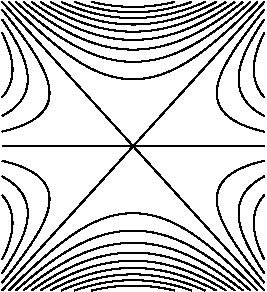
\includegraphics[width=0.308\textwidth, height=0.28\textwidth]{level3.pdf}
\quad
  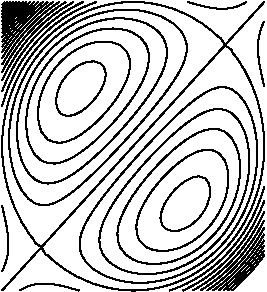
\includegraphics[width=0.308\textwidth, height=0.28\textwidth]{level1.pdf}
\end{center}
\begin{center}
  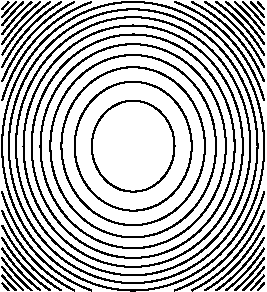
\includegraphics[width=0.308\textwidth, height=0.28\textwidth]{level4.pdf}
\quad
  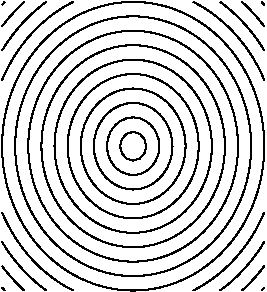
\includegraphics[width=0.308\textwidth, height=0.28\textwidth]{level2.pdf}
\end{center}
\end{question}

%\begin{hint}
%
%\end{hint}

\begin{answer}
(a)
\renewcommand{\arraystretch}{1.3}
     \begin{tabular}{|c|c|}
     \hline
    $\Atop{\text{critical}}{\text{point}}$  & type \\    
    \hline
     $(\frac{3}{2},-\frac{1}{4})$  & local min  \\ \hline
     $(-1,1)$    & saddle point \\  \hline
     \end{tabular}

(b)
\begin{center}
%(i)   \raisebox{-0.5\height}{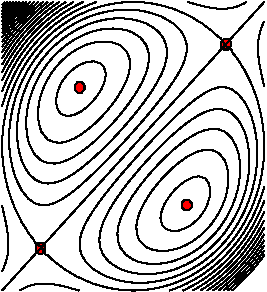
\includegraphics{level1b.pdf}}
(i)   \raisebox{-0.5\height}{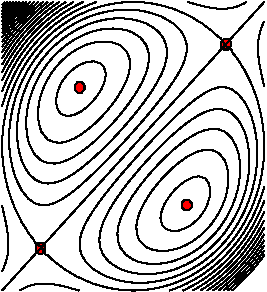
\includegraphics[width=0.33\textwidth, height=0.3\textwidth]{level1b.pdf}}
\quad
%(ii)  \raisebox{-0.5\height}{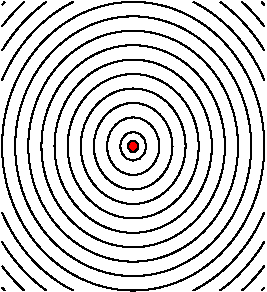
\includegraphics{level2b.pdf}}
(ii)  \raisebox{-0.5\height}{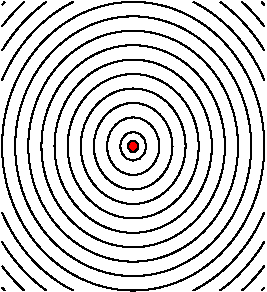
\includegraphics[width=0.33\textwidth, height=0.3\textwidth]{level2b.pdf}}
\end{center}
\begin{center}
(iii)   \raisebox{-0.5\height}{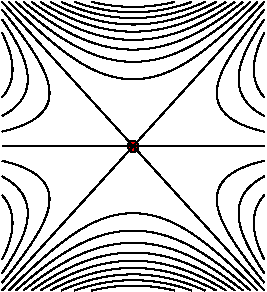
\includegraphics[width=0.33\textwidth, height=0.3\textwidth]{level3b.pdf}}
%(iii)   \raisebox{-0.5\height}{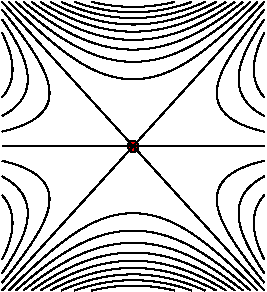
\includegraphics{level3b.pdf}}
\quad
%(iv)   \raisebox{-0.5\height}{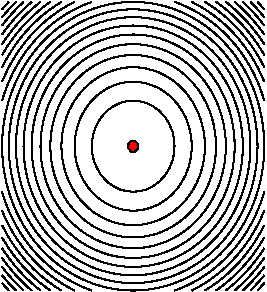
\includegraphics{level4b.pdf}}
(iv)   \raisebox{-0.5\height}{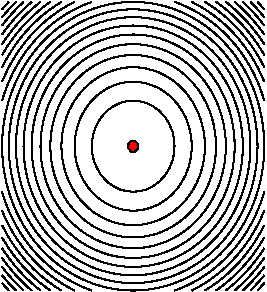
\includegraphics[width=0.33\textwidth, height=0.3\textwidth]{level4b.pdf}}
\end{center}
\end{answer}

\begin{solution}
(a)
To find the critical points we will need the
gradient of $f$ and to apply the second derivative test of 
Theorem \eref{CLP200}{thm second deriv test} in the CLP-3 text 
we will need all 
second order partial derivatives. So we need all partial derivatives of
$f$ up to order two.
Here they are.
\begin{alignat*}{3}
f&=x^3 + 3xy + 3y^2 - 6x - 3y - 6 \hidewidth\\
f_x&=3x^2+3y-6   & f_{xx}&=6x \qquad & f_{xy}&= 3\\
f_y&=3x+6y-3 \qquad & f_{yy}&=6\qquad & f_{yx}&= 3
\end{alignat*}

The critical points are the solutions of
\begin{equation*}
f_x=3x^2+3y-6=0   \qquad
f_y=3x+6y-3 = 0
\end{equation*}
Subtracting the second equation from $2$ times the first equation gives
\begin{equation*}
6x^2-3x-9=0
\iff
3(2x-3)(x+1)=0
\iff x=\frac{3}{2},\ -1
\end{equation*}
Since $y=\frac{1-x}{2}$ (from the second equation),
the critical points are $(\frac{3}{2},-\frac{1}{4})$, $(-1,1)$ and 
the classification is
\begin{center}
\renewcommand{\arraystretch}{1.3}
     \begin{tabular}{|c|c|c|c|}
     \hline
    $\Atop{\text{critical}}{\text{point}}$  & $f_{xx}f_{yy}-f_{xy}^2$ & 
                                                          $f_{xx}$ & type \\    
    \hline
     $(\frac{3}{2},-\frac{1}{4})$  & $(9)\times(6)-(3)^2> 0$ & $9$   
                       & local min  \\ \hline
     $(-1,1)$  & $(-6)\times (6)-(3)^2<0$ &   & saddle point \\  \hline
     \end{tabular}
\renewcommand{\arraystretch}{1.0}
\end{center}

(b) Both of the functions  $f(x, y) = \sqrt{x^2 + y^2}$ (i.e. (ii))
and  $f(x, y) = x^2 + y^2$ (i.e. (iv)) are invariant under rotations
around the $(0,0)$. So their level curves are circles centred on 
the origin. In polar coordinates $\sqrt{x^2 + y^2}$ is $r$. 
So the sketched level curves of the function in (ii) are
$r = 0, 0.1, 0.2, \ldots , 1.9, 2$. They are equally spaced.
So at this point, we know that the third picture goes with (iv)
and the fourth picture goes with (ii).

Notice that the lines $x=y$, $x=-y$ and $y=0$ are all level curves
of the function $f(x, y) = y(x + y)(x - y) + 1$ (i.e. of (iii))
with $f=1$. So the first picture goes with (iii). And the second picture
goes with (i).

Here are the pictures with critical points marked on them.
There are saddle points where level curves cross and there
are local max's or min's at ``bull's eyes''.
\begin{center}
%(i)   \raisebox{-0.5\height}{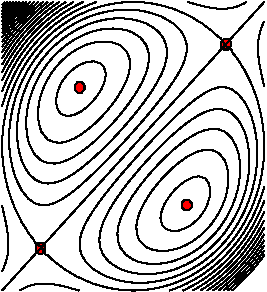
\includegraphics{level1b.pdf}}
(i)   \raisebox{-0.5\height}{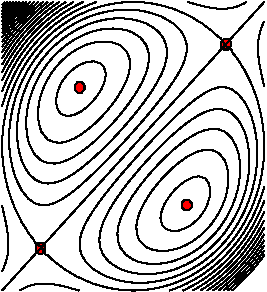
\includegraphics[width=0.33\textwidth, height=0.3\textwidth]{level1b.pdf}}
\quad
%(ii)  \raisebox{-0.5\height}{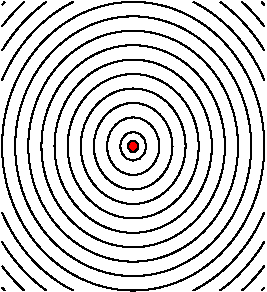
\includegraphics{level2b.pdf}}
(ii)  \raisebox{-0.5\height}{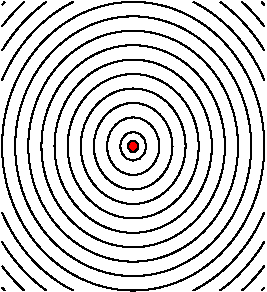
\includegraphics[width=0.33\textwidth, height=0.3\textwidth]{level2b.pdf}}
\end{center}
\begin{center}
(iii)   \raisebox{-0.5\height}{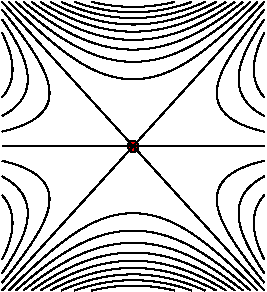
\includegraphics[width=0.33\textwidth, height=0.3\textwidth]{level3b.pdf}}
%(iii)   \raisebox{-0.5\height}{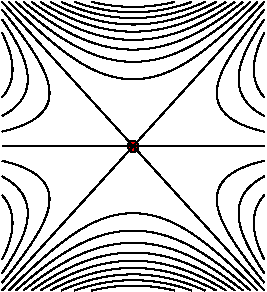
\includegraphics{level3b.pdf}}
\quad
%(iv)   \raisebox{-0.5\height}{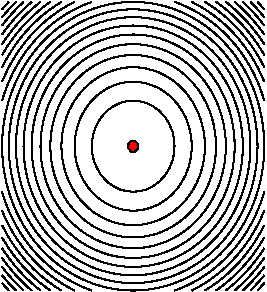
\includegraphics{level4b.pdf}}
(iv)   \raisebox{-0.5\height}{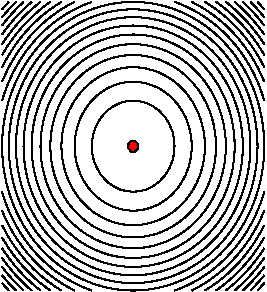
\includegraphics[width=0.33\textwidth, height=0.3\textwidth]{level4b.pdf}}
\end{center}
\end{solution}

%%%%%%%%%%%%%%%%%%%%%%%%%%%%%%%%
\begin{question}[M200 2010D] %4a
Let the function
\begin{equation*}
f(x,y) = x^3+3xy+3y^2-6x-3y-6
\end{equation*}
Classify as $\big[$local maxima, minima or saddle points$\big]$
all critical points of $f(x,y)$.
\end{question}

%\begin{hint}
%
%\end{hint}

\begin{answer}
\begin{center}
\renewcommand{\arraystretch}{1.3}
     \begin{tabular}{|c|c|}
     \hline
    $\Atop{\text{critical}}{\text{point}}$   & type \\    
    \hline
     $\big(\frac{3}{2},-\frac{1}{4}\big)$  & local min  \\ \hline
     $(-1,1)$  &  saddle point \\  \hline
     \end{tabular}
\renewcommand{\arraystretch}{1.0}
\end{center}
\end{answer}

\begin{solution}
To find the critical points we will need the
gradient of $f$, and to apply the second derivative test of 
Theorem \eref{CLP200}{thm second deriv test} in the CLP-3 text 
we will need all 
second order partial derivatives. So we need all partial derivatives of
$f$ up to order two.
Here they are.
\begin{alignat*}{3}
f&=x^3+3xy+3y^2-6x-3y-6 \hidewidth\\
f_x&=3x^2+3y-6   & f_{xx}&=6x \qquad & f_{xy}&= 3\\
f_y&=3x+6y-3 \qquad & f_{yy}&=6\qquad & f_{yx}&= 3
\end{alignat*}
(Of course, $f_{xy}$ and $f_{yx}$ have to be the same. It is still
useful to compute both, as a way to catch some mechanical errors.)

The critical points are the solutions of
\begin{alignat*}{3}
f_x&=3x^2+3y-6&&=0  \tag{E1} \\
f_y&=3x\ +6y-3 &&= 0  \tag{E2}
\end{alignat*}
Subtracting equation (E2) from twice equation (E1) gives
\begin{align*}
6x^2-3x-9=0
\iff (2x-3)(3x+3)=0
\end{align*}
So we must have either $x=\frac{3}{2}$ or $x=-1$.
\begin{itemize}
\item 
If $x=\frac{3}{2}$, (E2) reduces to $\frac{9}{2}+6y-3=0$ so $y=-\frac{1}{4}$.
\item 
If $x=-1$, (E2) reduces to $-3+6y-3=0$ so $y=1$.
\end{itemize}
So there are two critical points: $\big(\frac{3}{2},-\frac{1}{4}\big)$ and
$(-1,1)$.


The classification is
\begin{center}
\renewcommand{\arraystretch}{1.3}
     \begin{tabular}{|c|c|c|c|}
     \hline
    $\Atop{\text{critical}}{\text{point}}$  & $f_{xx}f_{yy}-f_{xy}^2$ & 
                                                          $f_{xx}$ & type \\    
    \hline
     $\big(\frac{3}{2},-\frac{1}{4}\big)$  & $(9)\times (6)-(3)^2> 0$ &  $9$  & local min  \\ \hline
     $(-1,1)$  & $(-6)\times (6)-(3)^2<0$ &  & saddle point \\  \hline
     \end{tabular}
\renewcommand{\arraystretch}{1.0}
\end{center}
 \end{solution}

%%%%%%%%%%%%%%%%%%%%%%%%%%%%%%%%
\begin{question}[M200 2011A] %5a,b
Let $h(x, y) = y(4 - x^2 - y^2)$.
\begin{enumerate}[(a)]
\item
Find and classify the critical points of $h(x, y)$ as local maxima, local minima or 
saddle points.
\item
Find the maximum and minimum values of $h(x, y)$ on the disk $x^2 + y^2 \le 1$.
\end{enumerate}
\end{question}

%\begin{hint}
%
%\end{hint}

\begin{answer}
(a)
\begin{center}
\renewcommand{\arraystretch}{1.3}
     \begin{tabular}{|c|c|}
     \hline
    $\Atop{\text{critical}}{\text{point}}$   & type \\    
    \hline
     $\left(0,\frac{2}{\sqrt{3}}\right)$  
            & local max  \\ \hline
     $\left(0,-\frac{2}{\sqrt{3}}\right)$  
            & local min \\  \hline
     $(2,0)$   & saddle point \\  \hline
     $(-2,0)$  & saddle point \\  \hline
     \end{tabular}
\renewcommand{\arraystretch}{1.0}
\end{center}

(b) The maximum and minimum values of $h(x,y)$ in $x^2+y^2\le 1$
     are $3$ (at $(0,1)$) and  $-3$ (at $(0,-1)$), respectively.
\end{answer}

\begin{solution}
(a)
To find the critical points we will need the
gradient of $h$ and to apply the second derivative test of 
Theorem \eref{CLP200}{thm second deriv test} in the CLP-3 text 
we will need all 
second order partial derivatives. So we need all partial derivatives of
$f$ up to order two.
Here they are.
\begin{alignat*}{3}
h&=y(4 - x^2 - y^2) \hidewidth\\
h_x&=-2xy   & h_{xx}&=-2y \qquad & h_{xy}&= -2x\\
h_y&=4-x^2-3y^2 \qquad & h_{yy}&=-6y\qquad & h_{yx}&= -2x
\end{alignat*}
(Of course, $h_{xy}$ and $h_{yx}$ have to be the same. It is still
useful to compute both, as a way to catch some mechanical errors.)

The critical points are the solutions of
\begin{equation*}
h_x=-2xy=0   \qquad
h_y=4-x^2-3y^2 = 0
\end{equation*}
The first equation is satisfied if at least one of $x=0$, $y=0$
are satisfied.
\begin{itemize}
\item 
If $x=0$, the second equation reduces to $4-3y^2=0$, which is
satisfied if $y=\pm\frac{2}{\sqrt{3}}$.
\item 
If $y=0$, the second equation reduces to $4-x^2=0$
which is satisfied if $x=\pm 2$.
\end{itemize}
So there are four critical points: 
   $\left(0,\frac{2}{\sqrt{3}}\right)$, $\left(0,-\frac{2}{\sqrt{3}}\right)$, 
   $(2,0)$, $(-2,0)$.


The classification is
\begin{center}
\renewcommand{\arraystretch}{1.3}
     \begin{tabular}{|c|c|c|c|}
     \hline
    $\Atop{\text{critical}}{\text{point}}$  & $h_{xx}h_{yy}-h_{xy}^2$ & 
                                                          $h_{xx}$ & type \\    
    \hline
     $\left(0,\frac{2}{\sqrt{3}}\right)$  
            & $\left(\frac{-4}{\sqrt{3}}\right)\times 
               \left(-\frac{12}{\sqrt{3}}\right)-(0)^2> 0$ 
           & $\frac{-4}{\sqrt{3}}$  & local max  \\ \hline
     $\left(0,-\frac{2}{\sqrt{3}}\right)$  
            & $\left(\frac{4}{\sqrt{3}}\right)\times 
                \left(\frac{12}{\sqrt{3}}\right)-(0)^2>0$ 
            & $\frac{4}{\sqrt{3}}$  & local min \\  \hline
     $(2,0)$  & $0\times 0-(-4)^2<0$ &   & saddle point \\  \hline
     $(-2,0)$  & $0\times 0-(4)^2<0$ &   & saddle point \\  \hline
     \end{tabular}
\renewcommand{\arraystretch}{1.0}
\end{center}

(b) The absolute max and min can occur either in the interior
    of the disk or on the boundary of the disk. The boundary
    of the disk is the circle $x^2+y^2=1$.
\begin{itemize}
\item Any absolute max or min in the interior of the disk
      must also be a local max or min and, since there are no
      singular points, must also be a critical point of $h$.
      We found all of the critical points of $h$ in part (a).
      Since $2>1$ and $\frac{2}{\sqrt{3}}>1$ none of the critical
      points are in the disk.
\item At each point of $x^2+y^2=1$ we have 
           $h(x,y)=3y$ 
           with $-1\le y\le 1$. Clearly the maximum value is $3$
           (at $(0,1)$) and the minimum value is $-3$ (at $(0,-1)$). 
\end{itemize}
So all together, the maximum and minimum values of $h(x,y)$ in $x^2+y^2\le 1$
     are $3$ (at $(0,1)$) and  $-3$ (at $(0,-1)$), respectively.
\end{solution}

%%%%%%%%%%%%%%%%%%%%%%%%%%%%%%%%
\begin{question}[M200 2012D] %4
Find the absolute maximum and minimum
values of the function
$f(x, y) = 5 + 2x - x^2 - 4y^2$ on the rectangular region 
\begin{equation*}
R = \Set{(x, y)}{ -1 \le x \le 3,\  -1 \le y \le 1}
\end{equation*}
\end{question}

%\begin{hint}
%
%\end{hint}

\begin{answer}
The minimum is $-2$ and the maximum is $6$.
\end{answer}

\begin{solution}
The maximum and minimum must either occur at a critical point or on
the boundary of $R$.
\begin{itemize}
\item 
The critical points are the solutions of
\begin{align*}
0&=f_x(x,y) = 2-2x \\
0&=f_y(x,y) = -8y \\ 
\end{align*} 
So the only critical point is $(1,0)$.
\item
On the side $x=-1$, $-1\le y\le 1$ of the boundary of $R$
\begin{equation*}
f(-1,y) = 2-4y^2 
\end{equation*}
This function decreases as $|y|$ increases. So its maximum value
on $-1\le y\le 1$ is achieved at $y=0$ and its minimum value is achieved
at $y=\pm 1$.

\item
On the side $x=3$, $-1\le y\le 1$ of the boundary of $R$
\begin{equation*}
f(3,y) = 2-4y^2 
\end{equation*}
This function decreases as $|y|$ increases. So its maximum value
on $-1\le y\le 1$ is achieved at $y=0$ and its minimum value is achieved
at $y=\pm 1$.

\item
On both sides $y=\pm 1$, $-1\le x\le 3$ of the boundary of $R$
\begin{equation*}
f(x,\pm 1) = 1+2x-x^2 = 2 -(x-1)^2 
\end{equation*}
This function decreases as $|x-1|$ increases. So its maximum value
on $-1\le x\le 3$ is achieved at $x=1$ and its minimum value is achieved
at $x= 3$ and $x=-1$ (both of whom are a distance $2$ from $x=1$).

\end{itemize}
So we have the following candidates for the locations of the min and max
\begin{center}
\renewcommand{\arraystretch}{1.3}
     \begin{tabular}{|c|c|c|c|c|c|c|}
     \hline
       point
       &$(1,0)$
       &$(-1,0)$ 
       &$(1,\pm 1)$ 
       &$(-1,\pm 1)$ 
       &$(3,0)$ 
       &$(3,\pm 1)$ \\ \hline
       value of $f$
       &$6$
       &$2$
       &$2$
       &$-2$
       &$2$
       &$-2$ \\ \hline
       &max 
       &    
       &  
       &min  
       &  
       &min \\ \hline
     \end{tabular}
\renewcommand{\arraystretch}{1.0}
\end{center}
So the minimum is $-2$ and the maximum is $6$.
\end{solution}

\begin{question}[M200 2013D] %4
Find the minimum of the function $h(x,y) = -4x - 2y + 6$ on the closed 
bounded domain defined by $x^2 + y^2 \le 1$.
\end{question}

%\begin{hint}
%
%\end{hint}

\begin{answer}
$6-2\sqrt{5}$
\end{answer}

\begin{solution}
Since $\vnabla h = \llt -4\,,\,-2 \rgt$ is never zero,
$h$ has no critical points and the minimum of $h$ on the disk
$x^2+y^2\le 1$ must be taken on the boundary, $x^2+y^2=1$,  of the
disk. To find the minimum on the boundary, we parametrize $x^2+y^2\le 1$
by $x=\cos\theta$, $y=\sin\theta$ and find the minimum of
\begin{align*}
H(\theta) = -4\cos\theta -2\sin\theta +6
\end{align*}  
Since 
\begin{align*}
0=H'(\theta) = 4\sin\theta -2\cos\theta
\implies 
x=\cos\theta = 2\sin\theta =2y
\end{align*}
So
\begin{align*}
1=x^2+y^2 = 4y^2 +y^2 =5 y^2
\implies y = \pm\frac{1}{\sqrt{5}},\ 
         x = \pm\frac{2}{\sqrt{5}}
\end{align*}
At these two points
\begin{align*}
h = 6-4x-2y = 6 - 10y =6 \mp \frac{10}{\sqrt{5}} =6 \mp 2\sqrt{5}
\end{align*}
The minimum is $6-2\sqrt{5}$.
\end{solution}

\begin{question}[M200 2014D] %5
Let $f(x,y) = xy(x + y - 3)$.
\begin{enumerate}[(a)]
\item
Find all critical points of $f$, and classify each one as a local maximum, 
a local minimum, or saddle point.
\item
Find the location and value of the absolute maximum and minimum of $f$ 
on the triangular region $x \ge 0$, $y \ge 0$, $x + y \le 8$.
\end{enumerate}
\end{question}

%\begin{hint}
%
%\end{hint}

\begin{answer}
(a) 
(0,0) and (3,0) and (0,3)  are saddle points\\
\phantom{(a) }(1,1) is a local min

(b)
The minimum is $-1$ at $(1,1)$ and the maximum is $80$ at $(4,4)$.
\end{answer}

\begin{solution}
(a)
Thinking a little way ahead, to find the critical points we will need the
gradient of $f$ and to apply the second derivative test of 
Theorem \eref{CLP200}{thm second deriv test} in the CLP-3 text 
we will need all 
second order partial derivatives. So we need all partial derivatives of
$f$ up to order two.
Here they are.
\begin{alignat*}{3}
f&=xy(x + y - 3) \hidewidth\\
f_x&=2xy+y^2-3y   & f_{xx}&=2y \qquad & f_{xy}&= 2x+2y-3\\
f_y&=x^2+2xy-3x \qquad & f_{yy}&=2x\qquad & f_{yx}&= 2x+2y-3
\end{alignat*}
(Of course, $f_{xy}$ and $f_{yx}$ have to be the same. It is still
useful to compute both, as a way to catch some mechanical errors.)

The critical points are the solutions of
\begin{equation*}
f_x=y(2x+y-3)=0   \qquad
f_y=x(x+2y-3) = 0
\end{equation*}
The first equation is satisfied if at least one of $y=0$, $y=3-2x$
are satisfied.
\begin{itemize}
\item 
If $y=0$, the second equation reduces to $x(x-3)=0$, which is
satisfied if either $x=0$ or $x=3$.
\item 
If $y=3-2x$, the second equation reduces to $x(x+6-4x-3)=x(3-3x)=0$
which is satisfied if $x=0$ or $x=1$.
\end{itemize}
So there are four critical points: $(0,0)$, $(3,0)$, $(0,3)$,
$(1,1)$.


The classification is
\begin{center}
\renewcommand{\arraystretch}{1.3}
     \begin{tabular}{|c|c|c|c|}
     \hline
    $\Atop{\text{critical}}{\text{point}}$  & $f_{xx}f_{yy}-f_{xy}^2$ & 
                                                          $f_{xx}$ & type \\    
    \hline
     $(0,0)$  & $0\times 0-(-3)^2< 0$ &    & saddle point  \\ \hline
     $(3,0)$  & $0\times 6-(3)^2<0$ &   & saddle point \\  \hline
     $(0,3)$  & $6\times 0-(3)^2<0$ &   & saddle point \\  \hline
     $(1,1)$  & $2\times 2-(1)^2>0$ & 2 & local min \\  \hline
     \end{tabular}
\renewcommand{\arraystretch}{1.0}
\end{center}

(b) The absolute max and min can occur either in the interior
    of the triangle or on the boundary of the triangle. The boundary
    of the triangle consists of the three line segments.
\begin{align*}
       L_1 &= \Set{(x,y)}{x=0,\ 0\le y\le 8} \\
       L_2 &= \Set{(x,y)}{y=0,\ 0\le x\le 8} \\
       L_3 &= \Set{(x,y)}{x+y=8,\ 0\le x\le 8} 
\end{align*}
\begin{itemize}
\item Any absolute max or min in the interior of the triangle
      must also be a local max or min and, since there are no
      singular points, must also be a critical point of $f$.
      We found all of the critical points of $f$ in part (a).
      Only one of them, namely $(1,1)$ is in the interior of the
      triangle. (The other three critical points are all on the
      boundary of the triangle.) We have $f(1,1) = -1$.
\item At each point of $L_1$ we have $x=0$ and so $f(x,y)=0$.
\item At each point of $L_2$ we have $y=0$ and so $f(x,y)=0$.
\item At each point of $L_3$ we have 
           $f(x,y)=x(8-x)(5)=40x-5x^2=5[8x-x^2]$ 
           with $0\le x\le 8$. As 
          $\diff{}{x}\big(40x-5x^2\big)= 40-10x$, the max and min of
         $40x-5x^2$ on $0\le x\le 8$ must be one of
         $5\big[8x-x^2\big]_{x=0}=0$ or
         $5\big[8x-x^2\big]_{x=8}=0$ or
         $5\big[8x-x^2\big]_{x=4}=80$. 
\end{itemize}
So all together, we have the following candidates for max and min, with the
max and min indicated.
\begin{center}
\renewcommand{\arraystretch}{1.3}
     \begin{tabular}{|c|c|c|c|c|c|c|}
     \hline
       point(s)
       &$(1,1)$
       &$L_1$
       &$L_2$
       &$(0,8)$ 
       &$(8,0)$ 
       &$(4,4)$ \\ \hline
       value of $f$
       &$-1$
       &$0$
       &$0$
       &$0$ 
       &$0$ 
       &$80$ \\ \hline
       &min
       & 
       & 
       & 
       & 
       & max\\ \hline
     \end{tabular}
\renewcommand{\arraystretch}{1.0}
\qquad
\raisebox{-0.5\height}{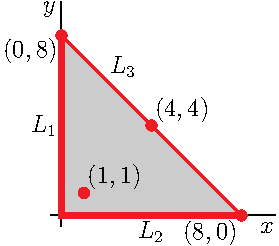
\includegraphics{OE14D_5.pdf}}
\end{center}
\end{solution}

%%%%%%%%%%%%%%%%%%%%%%%%%%%%%%%%
\begin{question}[M200 2015D] %4
Find and classify the critical points of 
$f(x,y) = 3x^2 y + y^3 - 3x^2 - 3y^2 + 4$.
\end{question}

%\begin{hint}
%
%\end{hint}

\begin{answer}
(0,0) is a local max

(0,2) is a local min

(1,1) and (-1,1) are saddle points
\end{answer}

\begin{solution}
Thinking a little way ahead, to find the critical points we will need the
gradient of $f$, and to apply the second derivative test of 
Theorem \eref{CLP200}{thm second deriv test} in the CLP-3 text 
we will need all 
second order partial derivatives. So we need all partial derivatives of
$f$ up to order two.
Here they are.
\begin{alignat*}{3}
f&=3x^2 y + y^3 - 3x^2 - 3y^2 + 4 \hidewidth\\
f_x&=6xy-6x   & f_{xx}&=6y-6 \qquad & f_{xy}&= 6x\\
f_y&=3x^2+3y^2-6y \qquad & f_{yy}&=6y-6\qquad & f_{yx}&= 6x
\end{alignat*}
(Of course, $f_{xy}$ and $f_{yx}$ have to be the same. It is still
useful to compute both, as a way to catch some mechanical errors.)

The critical points are the solutions of
\begin{equation*}
f_x=6x(y-1)=0   \qquad
f_y=3x^2+3y^2-6y = 0
\end{equation*}
The first equation is satisfied if at least one of $x=0$, $y=1$
are satisfied.
\begin{itemize}
\item 
If $x=0$, the second equation reduces to $3y^2-6y=0$, which is
satisfied if either $y=0$ or $y=2$.
\item 
If $y=1$, the second equation reduces to $3x^2 -3=0$
which is satisfied if $x=\pm 1$.
\end{itemize}
So there are four critical points: $(0,0)$, $(0,2)$, $(1,1)$,
$(-1,1)$.


The classification is
\begin{center}
\renewcommand{\arraystretch}{1.3}
     \begin{tabular}{|c|c|c|c|}
     \hline
    $\Atop{\text{critical}}{\text{point}}$  & $f_{xx}f_{yy}-f_{xy}^2$ & 
                                                          $f_{xx}$ & type \\    
    \hline
     $(0,0)$  & $(-6)\times (-6)-(0)^2> 0$ &  $-6$  & local max  \\ \hline
     $(0,2)$  & $6\times 6-(0)^2>0$ & 6 & local min \\  \hline
     $(1,1)$  & $0\times 0-(6)^2<0$ &   & saddle point \\  \hline
     $(-1,1)$  & $0\times 0-(-6)^2<0$ &  & saddle point \\  \hline
     \end{tabular}
\renewcommand{\arraystretch}{1.0}
\end{center}
 \end{solution}

%%%%%%%%%%%%%%%%%%%%%%%%%%%%%%%%
\begin{question}[M200 2004A] %4
Consider the function
\begin{equation*}
f(x,y)=2x^3 - 6xy + y^2 +4y 
\end{equation*}
\begin{enumerate}[(a)]
\item  
Find and classify all of the critical points of $f(x,y)$.
\item
Find the maximum and minimum values of $f(x,y)$ in the
triangle with vertices $(1,0)$, $(0,1)$ and $(1,1)$.  
\end{enumerate}
\end{question}

%\begin{hint}
%
%\end{hint}

\begin{answer}
(a) $(1,1)$ is a saddle point and $(2,4)$ is a local min

(b) The min and max  are $\frac{19}{27}$ and $5$, respectively.
\end{answer}

\begin{solution}
 (a) Since
\begin{alignat*}{5}
f&=2x^3 - 6xy + y^2 +4y \hidewidth \\
f_x&=6x^2-6y & f_{xx}&=12x\qquad && f_{xy}&= -6\\
f_y&=-6x+2y+4\qquad & f_{yy}&=2
\end{alignat*}
the critical points are the solutions of
\begin{alignat*}{5}
& & &f_x=0\qquad & &f_y=0 \\
&\iff\qquad& &y=x^2\qquad & &y-3x+2=0 \\
&\iff& &y=x^2 & &x^2-3x+2=0 \\
&\iff& &y=x^2 & &x=1\text{ or }2 
\end{alignat*}
So, there are two critical points: $(1,1),\ (2,4)$.
\begin{center}
\renewcommand{\arraystretch}{1.3}
     \begin{tabular}{|c|c|c|c|}
     \hline
    $\Atop{\text{critical}}{\text{point}}$  & $f_{xx}f_{yy}-f_{xy}^2$ & 
                                                          $f_{xx}$ & type \\    
    \hline
     $(1,1)$  & $12\times 2-(-6)^2<0$ &    & saddle point \\ \hline
     $(2,4)$  & $24\times 2-(-6)^2>0$ & $24$ & local min \\  \hline
     \end{tabular}
\renewcommand{\arraystretch}{1.0}
\end{center}

(b)
There are no critical points in the interior of the allowed region,
so both the maximum and the minimum occur only on the boundary. The boundary
consists of the line segments (i) $x=1$, $0\le y\le 1$, (ii) $y=1$, $0\le
x\le 1$ and (iii) $y=1-x$, $0\le x\le 1$.

\begin{center}
     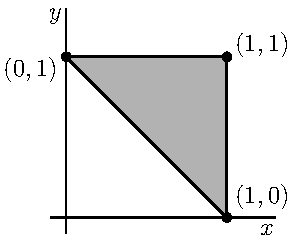
\includegraphics{OE04Q4.pdf}
\end{center}

\begin{itemize}
\item
First, we look at the part of the boundary with $x=1$. There $f=y^2-2y+2$.
As $\diff{}{y}(y^2-2y+2)=2y-2$ vanishes only at $y=1$, 
the max and min of $y^2-2y+2$ for $0\le y\le 1$ must occur either at $y=0$, 
where $f=2$, or at $y=1$, where $f=1$.

\item
Next, we look at the part of the boundary with $y=1$. There $f=2x^3-6x+5$.
As $\diff{}{x}(2x^3-6x+5)=6x^2-6$, 
the max and min of $2x^3-6x+5$ for $0\le x\le 1$ must occur either at $x=0$, 
where $f=5$, or at $x=1$, where $f=1$.

\item
Next, we look at the part of the boundary with $y=1-x$. There $f=2x^3-6x(1-x)
+(1-x)^2+4(1-x)=2x^3+7x^2-12x+5$.
As $\diff{}{x}(2x^3+7x^2-12x+5)=6x^2+14x-12
                               =2\big(3x^2+7x-6\big)
                               =2(3x-2)(x+3)$, 
the max and min of $2x^3+7x^2-12x+5$ for $0\le x\le 1$ must occur either at $x=0$, 
where $f=5$, or at $x=1$, where $f=2$, or at $x=\frac{2}{3}$, where $f=2(\frac{8}{27})-6(\frac{2}{3})(\frac{1}{3})+\frac{1}{9}+\frac{4}{3}
=\frac{16-36+3+36}{27}
=\frac{19}{27}$.
\end{itemize}
So all together, we have the following candidates for max and min, with the
max and min indicated.
\begin{center}
\renewcommand{\arraystretch}{1.3}
     \begin{tabular}{|c|c|c|c|c|}
     \hline
       point
       &$(1,0)$
       &$(1,1)$ 
       &$(0,1)$ 
       &$\big(\frac{2}{3},\frac{1}{3}\big)$ \\ \hline
       value of $f$
       &$2$
       &$1$
       &$5$
       &$\frac{19}{27}$\\ \hline
       & 
       & 
       & max
       & min\\ \hline
     \end{tabular}
\renewcommand{\arraystretch}{1.0}
\end{center}
\end{solution}

%%%%%%%%%%%%%%%%%%%%%%%%%%%%%%%
\begin{question}[M200 2003D] %4
Find all critical points of the function $f(x,y)=x^4+y^4-4xy+2$, 
and for each determine whether it is a local minimum, maximum
or saddle point.
\end{question}

%\begin{hint}
%
%\end{hint}

\begin{answer}
$(0,0)$ is a saddle point and $\pm(1,1)$ are local mins
\end{answer}

\begin{solution}
We have
\begin{alignat*}{5}
f(x,y)&=x^4+y^4-4xy+2\quad &
f_x(x,y)&=4x^3-4y\quad &
f_{xx}(x,y)&=12x^2
\\
 & & f_y(x,y)&=4y^3-4x &
f_{yy}(x,y)&=12y^2
\\
 & & & &f_{xy}(x,y)&=-4
\end{alignat*}
At a critical point
\begin{align*}
f_x(x,y)=f_y(x,y)=0
&\iff y=x^3\text{ and }x=y^3 \\
&\iff x=x^9\text{ and }y=x^3 \\
&\iff x(x^8-1)=0,\ y=x^3 \\
&\iff (x,y)=(0,0)\text{ or }(1,1)\text{ or }(-1,-1)
\end{align*}
Here is a table giving the classification of each of the three critical
points.

\begin{center}
\renewcommand{\arraystretch}{1.3}
     \begin{tabular}{|c|c|c|c|}
     \hline
    $\Atop{\text{critical}}{\text{point}}$  & $f_{xx}f_{yy}-f_{xy}^2$ & 
                                                          $f_{xx}$ & type \\    
    \hline
     $(0,0)$   & $0\times 0-(-4)^2<0$   &    & saddle point \\ \hline
     $(1,1)$   & $12\times 12-(-4)^2>0$ & 12 & local min \\  \hline
     $(-1,-1)$ & $12\times 12-(-4)^2>0$ & 12 & local min \\  \hline
     \end{tabular}
\renewcommand{\arraystretch}{1.0}
\end{center}
\end{solution}

%%%%%%%%%%%%%%%%%%%%%%%%%%%%%%%
\begin{question}[M200 2003A] %3
Let
\begin{equation*}
f(x,y)=xy(x+2y-6)
\end{equation*}
\begin{enumerate}[(a)]
\item
 Find every critical point of $f(x,y)$ and classify each one.
\item
 Let $D$ be the region in the plane between the hyperbola
$xy=4$ and the line $x+2y-6=0$. Find the maximum and minimum values of
$f(x,y)$ on $D$.
\end{enumerate}
\end{question}

%\begin{hint}
%
%\end{hint}

\begin{answer}
(a) $(0,0)$, $(6,0)$, $(0,3)$ are saddle points and $(2,1)$ is a local min

(b) The maximum value is $0$ and the minimum value is $4(4\sqrt{2}-6)
\approx -1.37$.
\end{answer}

\begin{solution}
(a) We have
\begin{alignat*}{5}
f(x,y)&=xy(x+2y-6)\quad &
     f_x(x,y)&=2xy+2y^2-6y\quad &
     f_{xx}(x,y)&=2y \\
 & & f_y(x,y)&=x^2+4xy-6x &
     f_{yy}(x,y)&=4x\\
 & & & &f_{xy}(x,y)&=2x+4y-6
\end{alignat*}
At a critical point
\begin{align*}
f_x(x,y)=f_y(x,y)=0
&\iff 2y(x+y-3)=0\text{ and }x(x+4y-6)=0 \\
&\iff \{y=0\text{ or }x+y=3\}\text{ and }\{x=0\text{ or }x+4y=6\}\\
&\iff \{x=y=0\}\text{ or }\{y=0,\ x+4y=6\}\\
&\hskip0.5in\text{ or }\{x+y=3,\ x=0\}
                   \text{ or }\{x+y=3,\ x+4y=6\}\\
&\iff (x,y)=(0,0)\text{ or }(6,0)\text{ or }(0,3)\text{ or }(2,1)
\end{align*}
Here is a table giving the classification of each of the four critical
points.
\begin{center}
\renewcommand{\arraystretch}{1.3}
     \begin{tabular}{|c|c|c|c|}
     \hline
    $\Atop{\text{critical}}{\text{point}}$  & $f_{xx}f_{yy}-f_{xy}^2$ & 
                                                          $f_{xx}$ & type \\    
    \hline
     $(0,0)$   & $0\times 0-(-6)^2<0$   &    &saddle point \\ \hline
     $(6,0)$   & $0\times 24-6^2<0$     &    &saddle point \\  \hline
     $(0,3)$   & $6\times 0-6^2<0$      &    &saddle point \\  \hline
     $(2,1)$   & $2\times 8-2^2>0$      & 2  &local min \\  \hline
     \end{tabular}
\renewcommand{\arraystretch}{1.0}
\end{center}

(b) Observe that $xy=4$ and $x+2y=6$ intersect when $x=6-2y$ and
\begin{align*}
(6-2y)y=4
&\iff 2y^2-6y+4=0
\iff 2(y-1)(y-2)=0 \\
&\iff (x,y) = (4,1)\text{ or }(2,2)
\end{align*}
The shaded region in the sketch below is $D$.
\begin{center}
     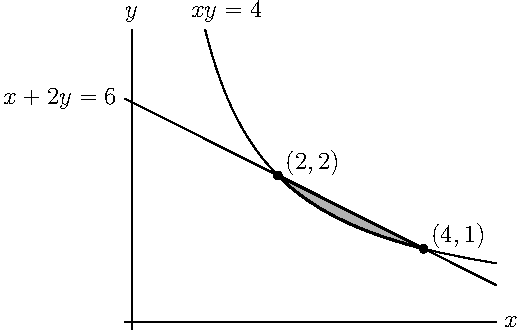
\includegraphics{OE03AQ3.pdf}
\end{center}
None of the critical points are in $D$. So the max and min must occur
at either $(2,2)$ or $(4,1)$ or on $xy=4$, $2<x<4$ (in which case
$F(x)=f\big(x,\frac{4}{x}\big)=4\big(x+\frac{8}{x}-6)$ obeys
$F'(x)=4-\frac{32}{x^2}=0\iff x=\pm2\sqrt{2}$) or on
$x+2y=6$, $2<x<4$ (in which case $f(x,y)$ is identically zero). So the
min and max must occur at one of 
\begin{center}
\renewcommand{\arraystretch}{1.3}
     \begin{tabular}{|c|c|}
     \hline
       $(x,y)$  & $f(x,y)$ \\ \hline
       $(2,2)$  & $2\times 2(2+2\times2-6)=0$ \\ \hline
       $(4,1)$  & $4\times 1(4+2\times 1-6)=0$ \\ \hline
       $(2\sqrt{2},\sqrt{2})$ & $4(2\sqrt{2}+2\sqrt{2}-6)<0$ \\ \hline 
     \end{tabular}
\renewcommand{\arraystretch}{1.0}
\end{center}
The maximum value is $0$ and the minimum value is $4(4\sqrt{2}-6)
\approx -1.37$.
\end{solution}

%%%%%%%%%%%%%%%%%%%%%%%%%%%%%%%%%%%%%%%%%
\begin{question} [M200 2002D] % 4
Find all the critical points of the function 
\begin{equation*}
f(x,y)=x^4+y^4-4xy
\end{equation*}
defined in the $xy$-plane. Classify each critical point as a local minimum, 
maximum or saddle point.
\end{question}

%\begin{hint}
%
%\end{hint}

\begin{answer}
$(0,0)$ is a saddle point and $\pm(1,1)$ are local mins
\end{answer}

\begin{solution}
We have
\begin{alignat*}{3}
f(x,y)&=x^4+y^4-4xy\qquad &
f_x(x,y)&=4x^3-4y\qquad &
f_{xx}(x,y)&=12x^2\\
 & & f_y(x,y)&=4y^3-4x &
f_{yy}(x,y)&=12y^2 \\
 & & & &f_{xy}(x,y)&=-4
\end{alignat*}
At a critical point
\begin{align*}
f_x(x,y)=f_y(x,y)=0
&\iff y=x^3\text{ and }x=y^3
\iff x=x^9\text{ and }y=x^3 \\
&\iff x(x^8-1)=0,\ y=x^3\\
&\iff (x,y)=(0,0)\text{ or }(1,1)\text{ or }(-1,-1)
\end{align*}
Here is a table giving the classification of each of the three critical
points.
\begin{center}
\renewcommand{\arraystretch}{1.3}
     \begin{tabular}{|c|c|c|c|}
     \hline
    $\Atop{\text{critical}}{\text{point}}$  & $f_{xx}f_{yy}-f_{xy}^2$ & 
                                                          $f_{xx}$ & type \\    
    \hline
     $(0,0)$   & $0\times 0-(-4)^2<0$   &    &saddle point \\ \hline
     $(1,1)$   & $12\times 12-(-4)^2>0$ & 12 & local min \\  \hline
     $(-1,-1)$ & $12\times 12-(-4)^2>0$ & 12 & local min \\  \hline
     \end{tabular}
\renewcommand{\arraystretch}{1.0}
\end{center}
\end{solution}

%%%%%%%%%%%%%%%%%%%%%%%%%%%%%%%%
\begin{question}[M200 2002A] %5
A metal plate is in the form of a semi-circular disc bounded
by the $x$-axis and the upper half of $x^2+y^2=4$. The temperature at
the point $(x,y)$ is given by $T(x,y)=\ln\big(1+x^2+y^2\big)-y$. Find the
coldest point on the plate, explaining your steps carefully. (Note: 
$\ln 2\approx 0.693$, $\ln 5\approx 1.609$)
\end{question}

%\begin{hint}
%\end{hint}

\begin{answer}
The coldest temperture is $-0.391$ and the coldest point is $(0,2)$.
\end{answer}

\begin{solution}
The coldest point must be either on the boundary of the plate
or in the interior of the plate. 
\begin{itemize}
\item 
On the semi--circular part of the boundary $0\le y\le 2$ and
$x^2+y^2=4$ so that $T=\ln\big(1+x^2+y^2\big)-y=\ln 5-y$. The smallest
value of $\ln 5-y$ is taken when $y$ is as large as possible, 
i.e. when $y=2$, and is $\ln 5 -2\approx -0.391$.

\item 
On the flat part of the boundary, $y=0$ and
$-2\le x\le 2$ so that $T=\ln\big(1+x^2+y^2\big)-y=\ln\big(1+x^2\big)$. 
The smallest value of $\ln\big(1+x^2\big)$ is taken when $x$ is as small as possible, i.e. when $x=0$, and is $0$.

\item 
If the coldest point is in the interior of the plate,
it must be at a critical point of $T(x,y)$. Since
\begin{align*}
T_x(x,y)=\frac{2x}{1+x^2+y^2}\qquad 
T_y(x,y)=\frac{2y}{1+x^2+y^2}-1
\end{align*}
a critical point must have $x=0$ and $\frac{2y}{1+x^2+y^2}-1=0$,
which is the case if and only if $x=0$ and $2y-1-y^2=0$. So the only 
critical point is $x=0,\ y=1$, where $T=\ln 2-1\approx -0.307$.
\end{itemize}
Since $-0.391<-0.307<0$, the coldest temperture is $-0.391$ and the
coldest point is $(0,2)$.
\end{solution}

%%%%%%%%%%%%%%%%%%%%%%%%%%%%%%%%
\begin{question}[M200 2001D] %4
Find all the critical points of the function 
\begin{equation*}
f(x,y)=x^3+xy^2-x
\end{equation*}
defined in the $xy$-plane. Classify each critical point as a local minimum,
 maximum or saddle point. Explain your reasoning.
\end{question}

%\begin{hint}
%
%\end{hint}

\begin{answer}
$(0,\pm 1)$ are saddle points,
$\big(\frac{1}{\sqrt{3}},0\big)$ is a local min and
$\big(-\frac{1}{\sqrt{3}},0\big)$ is a local max
\end{answer}

\begin{solution}
We have
\begin{alignat*}{3}
f(x,y)&=x^3+xy^2-x\qquad &
f_x(x,y)&=3x^2+y^2-1\qquad &
f_{xx}(x,y)&=6x \\
 & & f_y(x,y)&=2xy &
f_{yy}(x,y)&=2x \\
 & & & & f_{xy}(x,y)&=2y
\end{alignat*}
At a critical point
\begin{align*}
f_x(x,y)=f_y(x,y)=0
&\iff xy=0\text{ and }3x^2+y^2=1 \\
&\iff \{x=0\text{ or }y=0\}\text{ and }3x^2+y^2=1 \\
&\iff (x,y)=(0,1)\text{ or }(0,-1)\text{ or }\left(\frac{1}{\sqrt{3}},0\right)
\text{ or }\left(-\frac{1}{\sqrt{3}},0\right)
\end{align*}
Here is a table giving the classification of each of the four critical
points.
\begin{center}
\renewcommand{\arraystretch}{1.3}
     \begin{tabular}{|c|c|c|c|}
     \hline
    $\Atop{\text{critical}}{\text{point}}$  & $f_{xx}f_{yy}-f_{xy}^2$ & 
                                                          $f_{xx}$ & type \\    
    \hline
     $(0,1)$   & $0\times 0-2^2<0$      &    & saddle point \\ \hline
     $(0,-1)$  & $0\times 0-(-2)^2<0$   &    & saddle point \\  \hline
     $\big(\frac{1}{\sqrt{3}},0\big)$  &
           $2\sqrt{3}\times\frac{2}{\sqrt{3}}-0^2>0$ & $2\sqrt{3}$ & 
                                                     local min\\  \hline
     $\big(-\frac{1}{\sqrt{3}},0\big)$ & 
          $-2\sqrt{3}\times \big(-\frac{2}{\sqrt{3}}\big)-0^2>0$ &                                         $-2\sqrt{3}$ & local max \\ \hline
     \end{tabular}
\renewcommand{\arraystretch}{1.0}
\end{center}
\end{solution}

%%%%%%%%%%%%%%%%%%%%%%%%%%%%%%%%%%%%%%%%%
\begin{question} [M200 2001A] % 4
Consider the function 
$
g(x,y)=x^2-10y-y^2
.$ 
\begin{enumerate}[(a)]
\item
Find and classify  all critical points of $g$.

\item 
Find the absolute extrema of $g$ on the bounded region given by
\begin{equation*}
x^2+4y^2\le 16,\ y\le 0
\end{equation*}
\end{enumerate}
\end{question}

%\begin{hint}
%
%\end{hint}

\begin{answer}
(a) $(0,-5)$ is a saddle point

(b) The smallest value of $g$ is $0$ at $(0,0)$
and the largest value is $21$ at $(\pm 2\sqrt{3},-1)$.
\end{answer}

\begin{solution}
(a)
We have
\begin{alignat*}{5}
g(x,y)&=x^2-10y-y^2 \qquad&
g_x(x,y)&=2x \qquad&
g_{xx}(x,y)&=2\\
 & & g_y(x,y)&=-10-2y\qquad &
g_{yy}(x,y)&=-2 \\
 & & & &g_{xy}(x,y)&=0
\end{alignat*}
At a critical point
\begin{align*}
g_x(x,y)=g_y(x,y)=0
\iff 2x=0\text{ and }-10-2y=0
\iff (x,y)=(0,-5)
\end{align*}
Since $g_{xx}(0,-5)g_{yy}(0,-5)-g_{xy}(0,-5)^2=2\times(-2)-0^2<0$,
the critical point is a saddle point.

(b)
The extrema must be either on the boundary of the region
or in the interior of the region. 
\begin{itemize}
\item 
On the semi-elliptical part of the boundary $-2\le y\le 0$ 
and $x^2+4y^2=16$ so that $g=x^2-10y-y^2=16-10y-5y^2=21-5(y+1)^2$. This has 
a minimum value of 16 (at $y=0,-2$) and a maximum value of 21 (at $y=-1$).
You could also come to this conclusion by checking the critical point
of  $16-10y-5y^2$ (i.e. solving $\diff{}{y}(16-10y-5y^2)=0$)
and checking the end points of the allowed interval (namely $y=0$ and $y=-2$).

\item 
On the flat part of the boundary $y=0$ and
$-4\le x\le 4$ so that $g=x^2$.  
The smallest value is taken when $x=0$ and is $0$ and the largest value
is taken when $x=\pm 4$ and is $16$.
\item 
If an extremum is in the interior of the plate,
it must be at a critical point of $g(x,y)$. The only critical point is
not in the prescribed region.
\end{itemize}
Here is a table giving all candidates for extrema:
\begin{center}
\renewcommand{\arraystretch}{1.3}
     \begin{tabular}{|c|c|}
     \hline
       $(x,y)$  & $g(x,y)$ \\ \hline
       $(0,-2)$ & $16$ \\ \hline
       $(\pm 4,0)$ & $16$ \\ \hline
       $(\pm \sqrt{12},-1)$ & $21$ \\ \hline 
       $(0,0)$  & $0$ \\ \hline
     \end{tabular}
\renewcommand{\arraystretch}{1.0}
\end{center}
From the table the smallest value of $g$ is $0$ at $(0,0)$
and the largest value is $21$ at $(\pm 2\sqrt{3},-1)$.
\end{solution}

%%%%%%%%%%%%%%%%%%%%%%%%%%%%%%%%
\begin{question}[M200 2000D] %4
 Find and classify all critical points of
$$
f(x,y)=x^3-3xy^2-3x^2-3y^2
$$
\end{question}

%\begin{hint}
%
%\end{hint}

\begin{answer}
$(-1,\pm\sqrt{3})$ and $(2,0)$ are saddle points and 
$(0,0)$ is  a local max.
\end{answer}

\begin{solution}
We have
\begin{alignat*}{5}
f(x,y)&=x^3-3xy^2-3x^2-3y^2\qquad &
f_x(x,y)&=3x^2-3y^2-6x\qquad &
f_{xx}(x,y)&=6x-6 \\
 & & f_y(x,y)&=-6xy-6y &
f_{yy}(x,y)&=-6x-6 \\
 & & & &f_{xy}(x,y)&=-6y
\end{alignat*}
At a critical point
\begin{align*}
f_x(x,y)=f_y(x,y)=0
&\iff 3(x^2-y^2-2x)=0\text{ and }-6y(x+1)=0 \\
&\iff \{x=-1\text{ or }y=0\}\text{ and }x^2-y^2-2x=0 \\
&\iff (x,y)=(-1,\sqrt{3})\text{ or }(-1,-\sqrt{3})\text{ or }(0,0)
\text{ or }(2,0)
\end{align*}
Here is a table giving the classification of each of the four critical
points.
\begin{center}
\renewcommand{\arraystretch}{1.3}
     \begin{tabular}{|c|c|c|c|}
     \hline
    $\Atop{\text{critical}}{\text{point}}$  & $f_{xx}f_{yy}-f_{xy}^2$ & 
                                                          $f_{xx}$ & type \\    
    \hline
     $(0,0)$   & $(-6)\times(-6)-0^2>0$ & $-6$ & local max \\ \hline
     $(2,0)$   & $6\times(-18)-0^2<0$   &      & saddle point \\  \hline
  $(-1,\sqrt{3})$ & $(-12)\times0-(-6\sqrt{3})^2<0$ & & saddle point \\ \hline
  $(-1,-\sqrt{3})$ &$(-12)\times 0-(6\sqrt{3})^2<0$ & & saddle point \\ \hline
     \end{tabular}
\renewcommand{\arraystretch}{1.0}
\end{center}
\end{solution}

%%%%%%%%%%%%%%%%%%%%%%%%%%%%%%%%
\begin{question}[M200 2000A] %5
Find the maximum value of 
\begin{equation*}
f(x, y) = xye^{-(x^2 + y^2) / 2}
\end{equation*}
on the quarter-circle $D = \Set{(x, y)} { x^2 + y^2 \le 4,\ x\ge0,\ y\ge 0}$.
\end{question}

%\begin{hint}
%
%\end{hint}

\begin{answer}
$e^{-1}\approx0.368$
\end{answer}

\begin{solution}
The maximum must be either on the boundary of $D$ or in the interior of $D$.
\begin{itemize} 
\item On the circular part of the boundary $r=2$, 
      $0\le\theta\le\frac{\pi}{2}$ (in polar coordinates) so that 
$f=r^2\cos\theta\sin\theta e^{-r^2/2}=2\sin(2\theta)e^{-2}$. This has a maximum value 
of $2e^{-2}$ at $\theta=\frac{\pi}{4}$ or $x=y=\sqrt{2}$.
\item 
On the two flat parts of the boundary $x=0$ or $y=0$ so that $f=0$.  
\item
 If the maximum is in the interior of $D$,
it must be at a critical point of $f(x,y)$. Since
\begin{align*}
f_x(x,y)=e^{-(x^2 + y^2) / 2}\big[y-x^2y\big]\qquad
f_y(x,y)=e^{-(x^2 + y^2) / 2}\big[x-xy^2\big]
\end{align*}
$(x,y)$ is a critical point if and only if
\begin{align*}
&y(1-x^2)=0\text{ and }x(1-y^2)=0 \\
&\iff \{y=0\text{ or }x=1\text{ or }x=-1\}\text{ and }
       \{x=0\text{ or }y=1\text{ or }y=-1\}
\end{align*}
There are two critical points with $x,y\ge 0$, namely $(0,0)$ and $(1,1)$. 
The first of these is on the boundary of $D$ and the second is in the 
interior of $D$.
\end{itemize}
Here is a table giving all candidates for the maximum:
\begin{center}
\renewcommand{\arraystretch}{1.3}
     \begin{tabular}{|c|c|}
     \hline
       $(x,y)$  & $g(x,y)$ \\ \hline
       $(\sqrt{2},\sqrt{2})$ & $2e^{-2}\approx0.271$ \\ \hline
       $(x,0)$ & $0$ \\ \hline
       $(0,y)$ & $0$ \\ \hline
       $(1,1)$ & $e^{-1}\approx0.368$ \\ \hline
     \end{tabular}
\renewcommand{\arraystretch}{1.0}
\end{center}
Since $e>2$, we have that $2e^{-2}=e^{-1}\frac{2}{e}<e^{-1}$ and
the largest value is $e^{-1}$.
\end{solution}

%%%%%%%%%%%%%%%%%%%%%%%%%%%%%%%%
\begin{question}
Equal angle bends are made at equal distances from the two ends of a
100 metre long fence, so that the resulting three segment fence can be placed
along an existing wall to make an enclosure of trapezoidal shape. What
is the largest possible area for such an enclosure?
\end{question}

\begin{hint}
Suppose that the bends are made a  distance $x$ from the ends of the fence
and that the bends are through an angle $\theta$. Draw a sketch of the
enclosure and figure out its area, as a function of $x$ and $\theta$.
\end{hint}

\begin{answer}
$\frac{2500}{\sqrt{3}}$
\end{answer}

\begin{solution}
Suppose that the bends are made a  distance $x$ from the ends of the fence
and that the bends are through an angle $\theta$.
Here is a sketch of the enclosure.
\begin{center}
     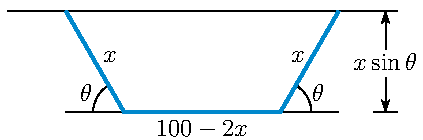
\includegraphics{fence.pdf}
\end{center}
It consists of a rectangle, with side lengths $100-2x$ and
$x\sin\theta$, together with two triangles, each of height $x\sin\theta$
and base length $x\cos\theta$. So the enclosure has area
\begin{align*}
A(x,\theta)&=(100-2x)x\sin\theta+2\cdot\half\cdot x\sin\theta\cdot x\cos\theta\\
&=(100x-2x^2)\sin\theta+\half x^2\sin(2\theta)
\end{align*}
The maximize the area, we need to solve
\begin{alignat*}{5}
0=A_x&=(100-4x)\sin\theta+x\sin(2\theta) & &\implies &
(100-4x)+2x\cos\theta&=0\cr
0=A_\theta&=(100x-2x^2)\cos\theta+x^2\cos(2\theta)\quad & &\implies\quad &
(100-2x)\cos\theta+x\cos(2\theta)&=0
\end{alignat*}
Here we have used that the fence of maximum area cannot have $\sin\theta=0$
or $x=0$, because in either of these two cases, the area enclosed will be zero. 
The first equation forces $\cos\theta=-\frac{100-4x}{2x}$
and hence $\cos(2\theta)=2\cos^2\theta-1=\frac{(100-4x)^2}{2x^2}-1$. 
Substituting these into the second equation gives
\begin{alignat*}{5}
& & -(100-2x)\frac{100-4x}{2x}+x\Big[\frac{(100-4x)^2}{2x^2}-1\Big]&=0 \\
&\implies & -(100-2x)(100-4x)+(100-4x)^2-2x^2&=0 \\
&\implies & 6x^2-200x&=0 \\
&\implies & x=\frac{100}{3}
\quad\cos\theta=-\frac{-100/3}{200/3}=\frac{1}{2}\quad
\theta&=60^\circ\\
& & A= \left(100\frac{100}{3}-2\frac{100^2}{3^2}\right)
             \frac{\sqrt{3}}{2}+\frac{1}{2} \frac{100^2}{3^2}\frac{\sqrt{3}}{2}
&=\frac{2500}{\sqrt{3}}
\end{alignat*}
\end{solution}

%%%%%%%%%%%%%%%%%%%%%%%%%%%%%%%%
\begin{question}
Find the most economical shape of a rectangular box that has
a fixed volume $V$ and that has no top.
\end{question}

\begin{hint}
Suppose that the box has side lengths $x$, $y$ and $z$.
\end{hint}

\begin{answer}
The box has dimensions $(2V)^{1/3}\times(2V)^{1/3}\times 2^{-2/3}V^{1/3}$.
\end{answer}

\begin{solution}
Suppose that the box has side lengths $x$, $y$ and $z$.
Here is a sketch.
\begin{center}
     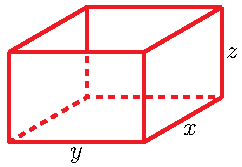
\includegraphics{box.pdf}
\end{center}
Because the box has to have volume $V$ we need that $V=xyz$.
We wish to minimize the area $A=xy+2yz+2xz$ of the four sides and bottom.
Substituting in $z=\frac{V}{xy}$,
\begin{align*}
A&=xy+2\frac{V}{x}+2\frac{V}{y}\\
A_x&=y-2\frac{V}{x^2}\\
A_y&=x-2\frac{V}{y^2}
\end{align*}
To minimize, we want $A_x=A_y=0$, which is the case when $yx^2=2V,\ xy^2=2V$.
This forces $yx^2=xy^2$. Since $V=xyz$ is nonzero, neither $x$ nor $y$
may be zero. So $x=y=(2V)^{1/3}$, $z=2^{-2/3}V^{1/3}$.
\end{solution}



%%%%%%%%%%%%%%%%%%
\subsection*{\Application}
%%%%%%%%%%%%%%%%%%

%%%%%%%%%%%%%%%%%%%%%%%%%%%%%%%%
\begin{question}[M200 2009D] %5
The temperature $T(x,y)$ at a point of the $xy$--plane is given by
\begin{equation*}
T(x,y) = 20 - 4x^2 - y^2 
\end{equation*}
\begin{enumerate}[(a)]
\item
Find the maximum and minimum values of $T(x,y)$ on the disk $D$ 
defined by $x^2 + y^2 \le 4$.

\item
Suppose an ant lives on the disk $D$. If the ant is initially at point 
$(1, 1)$, in which direction should it move so as to increase its 
temperature as quickly as possible?


\item
Suppose that the ant moves at a velocity $\vv = \llt -2, -1\rgt$. 
What is its rate of increase of temperature as it passes through $(1, 1)$?

\item 
Suppose the ant is constrained to stay on the curve $y = 2 - x^2$. 
Where should the ant go if it wants to be as warm as possible?

\end{enumerate}
\end{question}

%\begin{hint}
%
%\end{hint}

\begin{answer}
(a) The maximum and minimum values of $T(x,y)$ in $x^2+y^2\le 4$
     are $20$ (at $(0,0)$) and  $4$ (at $(\pm 2,0)$), respectively.

(b) $\frac{1}{\sqrt{17}}\llt -4,-1\rgt$\qquad
(c) $18$\qquad
(d) $(0,2)$
\end{answer}

\begin{solution}
(a)
The maximum and minimum can occur either in the interior
    of the disk or on the boundary of the disk. The boundary
    of the disk is the circle $x^2+y^2=4$.
\begin{itemize}
\item Any absolute max or min in the interior of the disk
      must also be a local max or min and, since there are no
      singular points, must also be a critical point of $h$.
      Since $T_x=-8x$ and $T_y=-2y$, the only critical point is
      $(x,y)=(0,0)$, where $T=20$.  Since $4x^2+y^2\ge 0$, 
      we have $T(x,y)=20-4x^2-y^2\le 20$. So the maximum value
      of $T$ (even in $\bbbr^2$) is $20$.    

\item At each point of $x^2+y^2=4$ we have 
           $T(x,y)=20-4x^2-y^2=20 -4x^2-(4-x^2)=16-3x^2$ 
           with $-2\le x\le 2$. So $T$ is a minimum when $x^2$ is a maximum.
           Thus the minimum value of $T$ on the disk is $16-3(\pm 2)^2=4$. 
\end{itemize}
So all together, the maximum and minimum values of $T(x,y)$ in $x^2+y^2\le 4$
     are $20$ (at $(0,0)$) and  $4$ (at $(\pm 2,0)$), respectively.

(b) To increase its temperature as quickly as possible, the ant should
    move in the direction of the temperature gradient
    $\vnabla T(1,1)=\llt -8x,-2y\rgt\Big|_{(x,y)=(1,1)}=\llt -8,-2\rgt$.
    A unit vector in that direction is $\frac{1}{\sqrt{17}}\llt -4,-1\rgt$. 

(c) The ant's rate f increase of temperature (per unit time) is
\begin{align*}
 \vnabla T(1,1)\cdot\llt -2,-1\rgt
=\llt -8,-2\rgt\cdot\llt -2,-1\rgt
=18
\end{align*}

(d) We are being asked to find the $(x,y)=(x,2-x^2)$ which maximizes
\begin{align*}
T\big(x,2-x^2\big) =20 -4x^2-\big(2-x^2\big)^2
                   = 16-x^4
\end{align*}
The maximum of $16-x^4$ is obviously $16$ at $x=0$. So the ant should
go to $\big(0,2-0^2\big)=(0,2)$.
\end{solution}


\begin{question}[M200 2014A] %3
Consider the function
\begin{equation*}
f (x,y) = 3kx^2 y + y^3 - 3x^2 - 3y^2 + 4
\end{equation*}
where $k > 0$ is a constant. 
Find and classify all critical points of $f(x,y)$ as local minima,
local maxima, saddle points or points of indeterminate type. 
Carefully distinguish the cases $k < \frac{1}{2}$, $k = \frac{1}{2}$ 
and $k > \frac{1}{2}$.
\end{question}

%\begin{hint}
%
%\end{hint}

\begin{answer}
\emph{Case $k<\frac{1}{2}$:\ \ \ }
\begin{center}
\renewcommand{\arraystretch}{1.3}
     \begin{tabular}{|c|c|}
     \hline
    $\Atop{\text{critical}}{\text{point}}$  & type \\    
    \hline
     $(0,0)$   & local max  \\ \hline
     $(0,2)$   & saddle point \\  \hline
     \end{tabular}
\renewcommand{\arraystretch}{1.0}
\end{center}


\emph{Case $k=\frac{1}{2}$:\ \ \ }
\begin{center}
\renewcommand{\arraystretch}{1.3}
     \begin{tabular}{|c|c|}
     \hline
    $\Atop{\text{critical}}{\text{point}}$  & type \\    
    \hline
     $(0,0)$   & local max  \\ \hline
     $(0,2)$   & unknown \\  \hline
     \end{tabular}
\renewcommand{\arraystretch}{1.0}
\end{center}

\emph{Case $k>\frac{1}{2}$:\ \ \ }
\begin{center}
\renewcommand{\arraystretch}{1.3}
     \begin{tabular}{|c|c|}
     \hline
    $\Atop{\text{critical}}{\text{point}}$   & type \\    
    \hline
     $(0,0)$    & local max  \\ \hline
     $(0,2)$    & local min \\  \hline
     $\left(\sqrt{\frac{1}{k^3}(2k-1)}\,,\,\frac{1}{k}\right)$  
                 & saddle point \\  \hline
     $\left(-\sqrt{\frac{1}{k^3}(2k-1)}\,,\,\frac{1}{k}\right)$  
                 & saddle point \\  \hline
     \end{tabular}
\renewcommand{\arraystretch}{1.0}
\end{center}
\end{answer}

\begin{solution}
To find the critical points we will need the
gradient of $f$ and to apply the second derivative test of 
Theorem \eref{CLP200}{thm second deriv test} in the CLP-3 text 
we will need all 
second order partial derivatives. So we need all partial derivatives of
$f$ up to order two.
Here they are.
\begin{alignat*}{3}
f&=3kx^2 y + y^3 - 3x^2 - 3y^2 + 4 \hidewidth\\
f_x&=6kxy-6x   & f_{xx}&=6ky-6 \qquad & f_{xy}&= 6kx\\
f_y&=3kx^2+3y^2-6y \qquad & f_{yy}&=6y-6\qquad & f_{yx}&= 6kx
\end{alignat*}
(Of course, $f_{xy}$ and $f_{yx}$ have to be the same. It is still
useful to compute both, as a way to catch some mechanical errors.)

The critical points are the solutions of
\begin{equation*}
f_x=6x(ky-1)=0   \qquad
f_y=3kx^2+3y^2-6y = 0
\end{equation*}
The first equation is satisfied if at least one of $x=0$, $y=\nicefrac{1}{k}$
are satisfied. (Recall that $k>0$.)
\begin{itemize}
\item 
If $x=0$, the second equation reduces to $3y(y-2)=0$, which is
satisfied if either $y=0$ or $y=2$.
\item 
If $y=\nicefrac{1}{k}$, the second equation reduces to 
$3kx^2+\frac{3}{k^2}-\frac{6}{k}=3kx^2+\frac{3}{k^2}(1-2k)=0$.
\end{itemize}

\emph{Case $k<\frac{1}{2}$:\ \ \ }
If $k<\frac{1}{2}$, then $\frac{3}{k^2}(1-2k)>0$ and the equation 
$3kx^2+\frac{3}{k^2}(1-2k)=0$ has no real solutions. In this case 
there are two critical points: $(0,0)$, $(0,2)$ and the classification is
\begin{center}
\renewcommand{\arraystretch}{1.3}
     \begin{tabular}{|c|c|c|c|}
     \hline
    $\Atop{\text{critical}}{\text{point}}$  & $f_{xx}f_{yy}-f_{xy}^2$ & 
                                                          $f_{xx}$ & type \\    
    \hline
     $(0,0)$  & $(-6)\times(-6)-(0)^2> 0$ & $-6$   & local max  \\ \hline
     $(0,2)$  & $(12k-6)\times 6-(0)^2<0$ &   & saddle point \\  \hline
     \end{tabular}
\renewcommand{\arraystretch}{1.0}
\end{center}


\emph{Case $k=\frac{1}{2}$:\ \ \ }
If $k=\frac{1}{2}$, then $\frac{3}{k^2}(1-2k)=0$ and the equation 
$3kx^2+\frac{3}{k^2}(1-2k)=0$ reduces to $3kx^2=0$ which has as its only solution $x=0$. We have already seen this third critical point, $x=0$, $y=\nicefrac{1}{k}=2$. 
So there are again two critical points: $(0,0)$, $(0,2)$ and 
the classification is
\begin{center}
\renewcommand{\arraystretch}{1.3}
     \begin{tabular}{|c|c|c|c|}
     \hline
    $\Atop{\text{critical}}{\text{point}}$  & $f_{xx}f_{yy}-f_{xy}^2$ & 
                                                          $f_{xx}$ & type \\    
    \hline
     $(0,0)$  & $(-6)\times(-6)-(0)^2> 0$ & $-6$   & local max  \\ \hline
     $(0,2)$  & $(12k-6)\times 6-(0)^2=0$ &   & unknown \\  \hline
     \end{tabular}
\renewcommand{\arraystretch}{1.0}
\end{center}

\emph{Case $k>\frac{1}{2}$:\ \ \ }
If $k>\frac{1}{2}$, then $\frac{3}{k^2}(1-2k)<0$ and the equation 
$3kx^2+\frac{3}{k^2}(1-2k)=0$ reduces to $3kx^2=\frac{3}{k^2}(2k-1)$ 
which has two solutions, namely $x=\pm\sqrt{\frac{1}{k^3}(2k-1)}$.  
So there are four critical points: $(0,0)$, $(0,2)$,
$\left(\sqrt{\frac{1}{k^3}(2k-1)}\,,\,\frac{1}{k}\right)$ and 
$\left(-\sqrt{\frac{1}{k^3}(2k-1)}\,,\,\frac{1}{k}\right)$ and 
the classification is
\begin{center}
\renewcommand{\arraystretch}{1.3}
     \begin{tabular}{|c|c|c|c|}
     \hline
    $\Atop{\text{critical}}{\text{point}}$  & $f_{xx}f_{yy}-f_{xy}^2$ & 
                                                          $f_{xx}$ & type \\    
    \hline
     $(0,0)$  & $(-6)\times(-6)-(0)^2> 0$ & $-6$   & local max  \\ \hline
     $(0,2)$  & $(12k-6)\times 6-(0)^2>0$ & $12k-6>0$ & local min \\  \hline
     $\left(\sqrt{\frac{1}{k^3}(2k-1)}\,,\,\frac{1}{k}\right)$  
               & $(6-6)\times (\frac{6}{k}-6)-(> 0)^2<0$ &   & saddle point \\  \hline
     $\left(-\sqrt{\frac{1}{k^3}(2k-1)}\,,\,\frac{1}{k}\right)$  
               & $(6-6)\times (\frac{6}{k}-6)-(< 0)^2<0$ &   & saddle point \\  \hline
     \end{tabular}
\renewcommand{\arraystretch}{1.0}
\end{center}
\end{solution}

%%%%%%%%%%%%%%%%%%%%%%%%%%%%%%%%
\begin{question}[M200 2002A] %3
\begin{enumerate}[(a)]
\item
Show that the function 
$f(x,y)=2x+4y+\frac{1}{xy}$
has exactly one critical point in the first quadrant $x>0$, $y>0$, and
find its value at that point.

\item 
Use the second derivative test to classify the critical point in part (a).

\item 
Hence explain why the inequality $2x+4y+\frac{1}{xy}\ge 6$ 
is valid for all positive real numbers $x$ and $y$.
\end{enumerate}
\end{question}

%\begin{hint}
%\end{hint}

\begin{answer}
(a) $x=1$, $y=\half$, $f\big(1,\half\big)=6$\qquad
(b) local minimum

(c) As $x$ or $y$ tends to infinity (with the other at least zero), 
$2x+4y$ tends to $+\infty$. As $(x,y)$ tends to any point on the first quadrant part of the $x$- and $y$--axes, $\frac{1}{xy}$ tends to $+\infty$.  
Hence as $x$ or $y$ tends to the boundary of the first quadrant 
(counting infinity as part of the boundary), $f(x,y)$ tends to $+\infty$. 
As a result $\big(1,\half\big)$ is a global (and not just local) minimum 
for $f$ in the first quadrant. Hence $f(x,y)\ge f\big(1,\half\big)=6$ 
for all $x,y>0$. 
\end{answer}

\begin{solution}
(a) For $x,y>0$,
\begin{align*}
f_x&=2-\frac{1}{x^2y}=0\iff y=\frac{1}{2x^2}\cr
f_y&=4-\frac{1}{xy^2}=0
\end{align*}
Substituting $y=\frac{1}{2x^2}$, from the first equation, into the second gives
$
4-4x^3=0
$
which forces $x=1$, $y=\half$. At $x=1$, $y=\half$,
\begin{equation*}
f\big(1,\half\big)=2+2+2=6
\end{equation*}

(b) The second derivatives are
\begin{equation*}
f_{xx}(x,y)=\frac{2}{x^3y}\qquad
f_{xy}(x,y)=\frac{1}{x^2y^2}\qquad
f_{yy}(x,y)=\frac{2}{xy^3}
\end{equation*}
In particular
\begin{equation*}
f_{xx}\big(1,\half\big)=4\qquad
f_{xy}\big(1,\half\big)=4\qquad
f_{yy}\big(1,\half\big)=16
\end{equation*}
Since $f_{xx}\big(1,\half\big)f_{yy}\big(1,\half\big)-
                 f_{xy}\big(1,\half\big)^2=4\times 16-4^2=48>0$ and $f_{xx}\big(1,\half\big)=4>0$,
the point $\big(1,\half\big)$ is a local minimum.

(c) As $x$ or $y$ tends to infinity (with the other at least zero), 
$2x+4y$ tends to $+\infty$. As $(x,y)$ tends to any point on the first quadrant part of the $x$- and $y$--axes, $\frac{1}{xy}$ tends to $+\infty$.  
Hence as $x$ or $y$ tends to the boundary of the first quadrant 
(counting infinity as part of the boundary), $f(x,y)$ tends to $+\infty$. 
As a result $\big(1,\half\big)$ is a global (and not just local) minimum 
for $f$ in the first quadrant. Hence $f(x,y)\ge f\big(1,\half\big)=6$ 
for all $x,y>0$. 
\end{solution}

%%%%%%%%%%%%%%%%%%%%%%%%%%%%%%%%
\begin{question}
An experiment yields data points $\ (x_i,y_i),\ i=1,2,\cdots,n.$ We wish to find the straight line $\ y=mx+b\ $ which ``best" fits the data. The definition of ``best" is ``minimizes the root mean square error", i.e. minimizes
$\ \sum_{i=1}^n (mx_i+b-y_i)^2$. Find $m$ and $b$.
\end{question}

%\begin{hint}
%\end{hint}

\begin{answer}
$m=\frac{nS_{xy}-S_xS_y}{nS_{x^2} -S_x^2}$ and
$b=\frac{S_yS_{x^2}-S_xS_{xy}}{nS_{x^2} -S_x^2}$ where
$S_y=\smsum\limits_{i=1}^n y_i$, $S_{x^2}=\smsum\limits_{i=1}^n x^2_i$ and
$S_{xy}=\smsum\limits_{i=1}^n x_iy_i$.
\end{answer}

\begin{solution}
We wish to choose $m$ and $b$ so as to minimize  the (square of the)
rms error $E(m,b)=\sum\limits_{i=1}^n (mx_i+b-y_i)^2$.
\begin{alignat*}{5}
0&=\pdiff{E}{m}&&=\smsum_{i=1}^n 2(mx_i+b-y_i)x_i
&&=m\Big[\smsum_{i=1}^n 2x^2_i\Big]+b\Big[\smsum_{i=1}^n 2x_i\Big]
-\Big[\smsum_{i=1}^n 2x_iy_i\Big]\\
0&=\pdiff{E}{b}&&=\smsum_{i=1}^n 2(mx_i+b-y_i)
&&=m\Big[\smsum_{i=1}^n 2x_i\Big]+b\Big[\smsum_{i=1}^n 2\Big]
-\Big[\smsum_{i=1}^n 2y_i\Big]
\end{alignat*}
There are a lot of symbols in those two equations. But remember that only two
of them, namely $m$ and $b$, are unknowns. All of the $x_i$'s and $y_i$'s are given data. We can make the equations look a lot less imposing if we define $S_x=\smsum_{i=1}^n x_i$, 
$S_y=\smsum_{i=1}^n y_i$, $S_{x^2}=\smsum_{i=1}^n x^2_i$ and
$S_{xy}=\smsum_{i=1}^n x_iy_i$. In terms of this notation, the two
 equations are (after dividing by two)
\begin{align*}
S_{x^2}\, m+S_x\, b&=S_{xy} \tag{\rm 1}\\
S_{x}\,m+n\,b&=S_{y} \tag{\rm 2}
\end{align*}
This is a system of two linear equations in two unknowns.
One way\footnote{This procedure is probably not the most efficient one. But it has the advantage that it always works, it does not require any ingenuity on the part of the solver, and it generalizes easily to larger linear systems of equations.} to solve them, is to use one of the two equations to solve
for one of the two unknowns in terms of the other unknown. For example,
equation (2) gives that
\begin{equation*}
b=\frac{1}{n}\big(S_y-S_x\,m\big)
\end{equation*}
If we now substitute this into equation (1) we get
\begin{equation*}
S_{x^2}\, m+\frac{S_x}{n}\big(S_y-S_x\,m\big)=S_{xy}
\implies \left(S_{x^2}-\frac{S_x^2}{n}\right)m = S_{xy} -\frac{S_xS_y}{n}
\end{equation*}
which is a single equation in the single unkown $m$. We can easily solve it for $m$. It tells us that
\begin{equation*}
m=\frac{nS_{xy}-S_xS_y}{nS_{x^2} -S_x^2}
\end{equation*}
Then substituting this back into $b=\frac{1}{n}\big(S_y-S_x\,m\big)$ gives us
\begin{equation*}
b=\frac{S_y}{n} 
      -\frac{S_x}{n}\left(\frac{nS_{xy}-S_xS_y}{nS_{x^2} -S_x^2}\right)
=\frac{S_yS_{x^2}-S_xS_{xy}}{nS_{x^2} -S_x^2}
\end{equation*}

\end{solution}

